% THIS IS SIGPROC-SP.TEX - VERSION 3.1
% WORKS WITH V3.2SP OF ACM_PROC_ARTICLE-SP.CLS
% APRIL 2009
%
% It is an example file showing how to use the 'acm_proc_article-sp.cls' V3.2SP
% LaTeX2e document class file for Conference Proceedings submissions.
% ----------------------------------------------------------------------------------------------------------------
% This .tex file (and associated .cls V3.2SP) *DOES NOT* produce:
%       1) The Permission Statement
%       2) The Conference (location) Info information
%       3) The Copyright Line with ACM data
%       4) Page numbering
% ---------------------------------------------------------------------------------------------------------------
% It is an example which *does* use the .bib file (from which the .bbl file
% is produced).
% REMEMBER HOWEVER: After having produced the .bbl file,
% and prior to final submission,
% you need to 'insert'  your .bbl file into your source .tex file so as to provide
% ONE 'self-contained' source file.
%
% Questions regarding SIGS should be sent to
% Adrienne Griscti ---> griscti@acm.org
%
% Questions/suggestions regarding the guidelines, .tex and .cls files, etc. to
% Gerald Murray ---> murray@hq.acm.org
%
% For tracking purposes - this is V3.1SP - APRIL 2009

%\documentclass{acm_proc_article-sp}  % mise en comment (19/01/2016)

\documentclass{sig-alternate-05-2015} % ajout (19/01/2016)

%%%\CopyrightYear{2016}
\setcopyright{acmlicensed}
\conferenceinfo{HSCC'17,}{April 17--20, 2017, Pittsburgh, Pennsylvania}
%\isbn{978-1-4503-3955-1/16/04}\acmPrice{\$15.00}
\doi{http://dx.doi.org/XXXX.XXXX}

%Authors, replace the red X's with your assigned DOI string.

\clubpenalty=10000
\widowpenalty = 10000


\usepackage{listings}
\usepackage{graphicx} % Required for including pictures
\usepackage{amsfonts}
\usepackage{amsmath}

\usepackage{tikz}
\usepgflibrary{plotmarks}
\usepgfmodule[plot]
\usepackage{pgfplots}
\usepackage{cite}
\usepackage{epsfig}
\usepackage{float} % Allows putting an [H] in \begin{figure} to specify the exact location of the figure
\usepackage{wrapfig} % Allows in-line images such as the example fish picture
%\usepackage{amsthm}
\usepackage{amssymb}
\usepackage{hyperref}
\usepackage{tikz}
\usepackage{multirow}
\usepackage{comment}
\usepackage[]{algorithm2e}
\usepackage{caption}
\usepackage{subcaption}
\usepackage{url}
% \font\dsrom=dsrom10 scaled 1200
% \def \ind{\textrm{\dsrom{1}}}

 \newcommand\ForAuthors[1]%          %  temporary remark for the
 {\par\smallskip                     %  authors:
  \begin{center}%                    %
   \fbox%                            %    --------
   {\parbox{0.9\linewidth}%          %    |  #1  |
    {\raggedright\sc--- #1}%         %    --------
   }%                                %
  \end{center}%                      %
  \par\smallskip                     %
 }        


\newcommand{\comm}[1]{}
\newtheorem{definition}{Definition}
\newtheorem{theorem}{Theorem}
\newtheorem{proposition}{Proposition}
\newtheorem{lemma}{Lemma}
\newtheorem{example}{Example}

\def\N{{\mathbb N}}
\def\Z{{\mathbb Z}}
\def\R{{\mathbb R}}
\def\intvl#1{\mbox{$[ #1 ]$}}

\newcommand{\IR}{\mathbb{IR}}
\newcommand{\va}{{\bf a}}
\newcommand{\vb}{{\bf b}}
\newcommand{\vc}{{\bf c}}
\newcommand{\vd}{{\bf d}}
\newcommand{\vf}{{\bf f}}
\newcommand{\vh}{{\bf h}}
\newcommand{\vg}{{\bf g}}
\newcommand{\vm}{{\bf m}}
\newcommand{\vu}{{\bf u}}
\newcommand{\vv}{{\bf v}}
\newcommand{\vx}{{\bf x}}
\newcommand{\vy}{{\bf y}}
\newcommand{\vt}{{\bf t}}
\newcommand{\vz}{{\bf z}}
\newcommand{\vJ}{{\bf J}}
\newcommand{\vA}{{\bf A}}
\newcommand{\vB}{{\bf B}}
\DeclareMathOperator{\interior}{int}
\newcommand{\inter}[1]{\left[#1\right]}
\DeclareMathOperator{\diag}{Diag}
\DeclareMathOperator{\offdiag}{OffDiag}
\DeclareMathOperator{\range}{range}
\usepackage{color}

\newcommand{\dual}{\mbox{dual }}
\newcommand{\pro}{\mbox{pro }}
\newcommand{\semb}{[ \! [}
\newcommand{\seme}{] \! ]}
%\newcommand{\comment2}[1]{}
\newcommand{\norma}[1]{\mbox{$\mid \! \mid #1 \mid \! \mid^a$}}
\newcommand{\normu}[1]{\mbox{$\mid \! \mid #1 \mid \! \mid^\cup$}}
\newcommand{\normn}[1]{\mbox{$\mid \! \mid #1 \mid \! \mid^\cap$}}
\newtheorem{sketch}{Sketch of proof.}
\newtheorem{problem}{Problem}
\newtheorem{property}{Property}
\def\ve{\vec{\varepsilon}}
\def\vp{\vec{\varphi}}
\def\ua{\uparrow_\circ}
\def\da{\downarrow_\circ}
\def\ra{\rightarrow}
\def\bbr{{\Bbb R}}
\def\bbf{{\Bbb F}}
\def\F{{\Bbb F}}
\def\A{{\Bbb A}}
\def\calD{{\Bbb D}}
\def\I{{\Bbb I \Bbb R}}
\def\K{{\Bbb I \Bbb K}}
%\def\RAff{{\Bbb R \Bbb A}}
\def\RAff{{\Bbb A \Bbb R}}
%\def\IAff{{\Bbb I \Bbb A}}
\def\IAff{{\Bbb A \Bbb I}}

\makeatletter
\newcommand\listofTODO{\section*{Remaining TODO}\@starttoc{tdo}}
\makeatother
\newcommand{\addTODO}[1]{\addcontentsline{tdo}{toc}{#1}}
\newcommand{\TODO}[1]{{\bf{\scriptsize #1}\addTODO{#1}}}
\newcommand{\SP}[1]{\TODO{Sylvie : #1}}
\newcommand{\EG}[1]{\TODO{Eric : #1}}

\definecolor{cof}{RGB}{219,144,71}
\definecolor{pur}{RGB}{186,146,162}
\definecolor{greeo}{RGB}{91,173,69}
\definecolor{greet}{RGB}{52,111,72}
\definecolor{red}{RGB}{210,0,32}

%\theoremstyle{remark}
\newtheorem{remark}{Remark}
\def\norm#1{\mbox{$\left\| #1 \right\|_1$}} 


\usetikzlibrary{positioning}
\tikzset{main node/.style={circle,fill=blue!20,draw,minimum size=0.8cm,inner sep=0pt},
            }

\begin{document}

\def\transpose#1{{}^t \! #1}
% boldface letters for intervals
\def\bfm#1{\protect{\makebox{\boldmath $#1$}}}
\def\a {\bfm{a}}
\def\b {\bfm{b}}
\def\c {\bfm{c}}
\def\d {\bfm{d}}
\def\e {\bfm{e}}
\def\f {\bfm{f}}
\def\g {\bfm{g}}
\def\h {\bfm{h}}
\def\ii {\bfm{i}}       % \i is already 'i without dot'
\def\j {\bfm{j}}
\def\k {\bfm{k}}
\def\l {\bfm{l}}
\def\m {\bfm{m}}
\def\n {\bfm{n}}
\def\o {\bfm{o}}
\def\p {\bfm{p}}
\def\q {\bfm{q}}
\def\r {\bfm{r}}
\def\s {\bfm{s}}
\def\t {\bfm{t}}
\def\u {\bfm{u}}
\def\vv {\bfm{v}}       % \v is already 'check' 
\def\w {\bfm{w}}
\def\x {\bfm{x}}
\def\y {\bfm{y}}
\def\z {\bfm{z}}
%\def\A {\bfm{A}}
\def\B {\bfm{B}}
\def\C {\bfm{C}}
\def\DD{\bfm{D}}        % \D is already \displaystyle
\def\E {\bfm{E}}
%\def\F {\bfm{F}}
\def\G {\bfm{G}}
\def\H {\bfm{H}}
%\def\I {\bfm{I}}
\def\J {\bfm{J}}
%\def\K {\bfm{K}}
\def\L {\bfm{L}}
\def\M {\bfm{M}}
\def\N {\bfm{N}}
\def\O {\bfm{O}}
\def\P {\bfm{P}}
\def\Q {\bfm{Q}}
%\def\R {\bfm{R}}
\def\S {\bfm{S}}
\def\T {\bfm{T}}
\def\U {\bfm{U}}
\def\V {\bfm{V}}
\def\W {\bfm{W}}
\def\X {\bfm{X}}
\def\Y {\bfm{Y}}


\title{Forward inner-approximated reachability  of non-linear continuous systems}
%\subtitle{[Extended Abstract]
%\titlenote{A full version of this paper is available as
%\textit{Author's Guide to Preparing ACM SIG Proceedings Using
%\LaTeX$2_\epsilon$\ and BibTeX} at
%\texttt{www.acm.org/eaddress.htm}}}
%
% You need the command \numberofauthors to handle the 'placement
% and alignment' of the authors beneath the title.
%
% For aesthetic reasons, we recommend 'three authors at a time'
% i.e. three 'name/affiliation blocks' be placed beneath the title.
%
% NOTE: You are NOT restricted in how many 'rows' of
% "name/affiliations" may appear. We just ask that you restrict
% the number of 'columns' to three.
%
% Because of the available 'opening page real-estate'
% we ask you to refrain from putting more than six authors
% (two rows with three columns) beneath the article title.
% More than six makes the first-page appear very cluttered indeed.
%
% Use the \alignauthor commands to handle the names
% and affiliations for an 'aesthetic maximum' of six authors.
% Add names, affiliations, addresses for
% the seventh etc. author(s) as the argument for the
% \additionalauthors command.
% These 'additional authors' will be output/set for you
% without further effort on your part as the last section in
% the body of your article BEFORE References or any Appendices.

\numberofauthors{2} %  in this sample file, there are a *total*
% of EIGHT authors. SIX appear on the 'first-page' (for formatting
% reasons) and the remaining two appear in the \additionalauthors section.
%
\author{
% You can go ahead and credit any number of authors here,
% e.g. one 'row of three' or two rows (consisting of one row of three
% and a second row of one, two or three).
%
% The command \alignauthor (no curly braces needed) should
% precede each author name, affiliation/snail-mail address and
% e-mail address. Additionally, tag each line of
% affiliation/address with \affaddr, and tag the
% e-mail address with \email.
%
% 1st. author
\alignauthor E. Goubault \\ %\titlenote{Dr.~Trovato insisted his name be first.}\\
       \affaddr{LIX, Ecole Polytechnique, CNRS, }\\
       \affaddr{Universit\'e Paris-Saclay, 91128 Palaiseau, France} \\
       \email{\small goubault@lix.polytechnique.fr}
% 2nd. author
\alignauthor S. Putot \\ %\titlenote{The secretary disavows any knowledge of this author's actions.}\\
       \affaddr{LIX, Ecole Polytechnique, CNRS, } \\
       \affaddr{Universit\'e Paris-Saclay, 91128 Palaiseau, France}\\
       \email{\small putot@lix.polytechnique.fr}
}
%\author{}

\maketitle
\begin{abstract}
We propose an approach for computing inner-approxima\-tions (also called under-approximations) of reachable sets of dynamical systems 
defined by non-linear, uncertain, ordinary differential equations. This is a notoriously difficult problem, much more intricate than 
outer-approximations (also called over-approx\-imations), for whi\-ch there exist well known solutions, mostly based on Taylor models. 
The few methods developed recently for inner-approximation mostly rely on backward flowmaps, and extra ingredients, either coming from optimization, 
or involving topological criteria, are required. Our solution, in comparison, builds on rather inexpensive set-based methods, namely a generalized
mean-value theorem combined with Taylor models outer-approximations of the flow and its Jacobian with respect 
to the uncertain inputs and parameters.
%for inner-approximations is also based on Taylor models, but contrarily to the few methods developped recently, 
% is a direct forward method, which only relies on rather inexpensive set-based methods, namely a generalized mean-value theorem 
%applied to 
% instead of the %clever, but still complicated, 
%existing  methods relying on backward flowmaps and for which extra ingredients, either coming from optimisation, or involving topological criteria, are required. 
We demonstrate with a C/C++ prototype implementation that our method is both efficient and
precise on classical examples. 
%\ForAuthors{Est-ce dangereux de se placer un peu sur la complexite? On pourrait nous reprocher d'avoir un
%nombre d'equations en le produit du nombre d'equations d'origine, avec le nombre de variables... Mais la methode
%de Sriram et celle des chinois est potentiellement tres complexe.}
%Our method, being based on Taylor models and being a forward method, also provides outer-approximations, naturally. 
The combination of such forward inner and outer Taylor-model based approximations 
can be used as a basis for the verification and falsification of properties
of cyber-physical systems. 
%- forward inner- and outer- approximations 
%of the set of  states reachable by an uncertain hybrid systems, that is with uncertain initial conditions and parameters.\\
%- little studied and difficult problem, the small number of existing approaches mostly attack the dual problem aof backward inner-apporximated reachability \\
%- based on a combination of Taylor based methids for teh solution of IVP and generalized mean value theorem for inner-approximation~\cite{hscc14}\\
%- experiments with matlab implementation
\end{abstract}

% A category with the (minimum) three required fields
% CATEGORIES A VERIFIER/REMPLIR, CELLES_CI SONT REPRISES d'HSCC PRECEDENTS
\category{F.1.1}{Theory of Computation}{Computation by Abstract Devices}%{Models of Computation}
\category{G.1.7}{Mathematics of Computing}{Numerical Analysis}%{Ordinary Differential Equations}
\category{G.1.0}{Numerical Analysis}{General}[Interval arithmetic,Numerical algorithms]
\category{G.4}{Mathematical Software}{Reliability and robustness}
%A category including the fourth, optional field follows...
%\category{...}{...}{...}[...]

\terms{Algorithms, Theory, Verification}

%\keywords{ACM proceedings, \LaTeX, text tagging} % NOT required for Proceedings
\keywords{Inner-approximation, Taylor models, affine arithmetic, modal intervals} % NOT required for Proceedings

%******************************************************************************
\section{Introduction}
%******************************************************************************
%
%\ForAuthors{Intro a reprendre: d'abord il manque les ref, mais surtout elle etait pas mal orientee systemes hybrides et prop temporelles, 
%on veut sans doute affaiblir ca}

%The verification of software-enabled real-time control systems requires reasoning about non-linear hybrid systems, 
%that exhibit both discrete and continuous behavior. Computing the reachable set of such systems is a central component 
%of model-checking. While the exact reachability problem for hybrid systems is generally undecidable, in the recent 
%years there has been much progress in the computation of outer-approximations of the reachable set, first for the 
%verification of affine hybrid systems~\cite{}, but also for the more general class of non-linear hybrid systems~\cite{}. 
%An outer-approximation makes possible the verification of safety properties of such systems. However, the verification 
%of more general temporal properties, such as viability~\cite{} properties for instance, or the falsification of safety properties, 
%also require inner-approximating the reachable set, that is computing set of states that are definitely reached, or put differently 
%flowpipes that contain only solutions of the uncertain system.

We propose an approach to compute inner-approxi\-mating flowpipes, that under-approximate reachable sets 
of uncertain continuous systems described by ordinary differential equations (ODEs), which 
are widely used for modeling all sorts of physical, biological and even economic or
social systems.  

While outer-approximations describe states that may be rea\-ched, inner-approximations represent
states that are actually reachable from one of the initial states. They are
thus a very useful complement to the more classical outer-approxima\-tions, since they allow to show
that some executions of the system will actually reach a target or a bad state. Also, the combination of
inner and outer-approximations allows for judging the quality of the abstractions involved. 
But methods for inner-approximated reachability are far less developed, and especially in the non-linear case, 
since most methods in the non-linear case rely on conservative linearizations, which necessarily produce outer approximations.

In this work, we concentrate on the inner-approximation of the reachable sets of
the continuous part of hybrid systems. %We intend to handle guard conditions in subsequent work.
%The discrete part has been treated elsewhere \cite{hscc14}
%and we intend to treat guards in subsequent work. 
We consider general systems of parametric ODEs, i.e. possibly non-linear, or
even non-polyno\-mial, of the form : 
\begin{equation}
\dot{x}(t) = f(x,p,t)
\label{eq:flow}
\end{equation}
\noindent where the continuous variables $x$ belong to a state-space domain 
${\cal D} \subseteq \R^n$, the (constant) parameters $p$ belong to the uncertainty domain
${\cal P} \subseteq \R^p$, and 
$f: {\cal D} \times {\cal P} \times \R^+ \rightarrow {\cal D}$ is assumed sufficiently smooth 
on ${\cal D} \subseteq \R^n$ (at least ${\cal C}^1$, and sometimes more when we will use higher
Taylor models, see Section \ref{sec:Taylor}).

Introducing the new state variable $z=(x,p,t)$ with $\dot z = (\dot x,0,1)$, and defining ${\cal Z} = {\cal D} \times {\cal P} \times \R^+$,
the equation (\ref{eq:flow}) can be rewritten with all uncertainties embedded in the initial state vector~:
\begin{equation} \dot z(t) = f(z)
\label{eq:flowb}
\end{equation}

In the sequel, we will write $x_i$ and $f_i$ for the $i$th component ($i=1,\ldots,n$) of
the state vector $x$ and of the function $f$. 

\paragraph{Contributions:}

This paper extends the work of ~\cite{sas07,hscc14}, where the authors proposed an approach for direct forward inner-approximated reachability of 
%\ForAuthors{Attention au double-blind review}
discrete dynamical systems, and gave a few hints to handle continuous and hybrid systems. 
%on this previous work. \\
We are computing here inner-approximations of the flow of uncertain initial value problems, as defined in Section \ref{prelim}. 
There are two main ingredients involved in our method. The first ingredient is that in order to derive inner-approximations, we only need forward 
outer-approxima\-tions of some dynamics, which we can compute using classical
Taylor models, introduced in Section \ref{sec:Taylor}. But we need to outer-approximate not only 
the set of reachable states of the dynamics but also
of the variational equations, including the dynamics of the Jacobian of the flow with respect to the uncertain
initial values. 

The second main ingredient of our method is 
a generalized mean value theorem, that we introduce in Section \ref{generalizedmean}, applied to the flow of the uncertain ODE. 
The generalized mean value theorem relies itself on modal intervals, a simple 
extension of classical interval arithmetic (see Section \ref{Kaucherar}), to inner-approximate 
the image of an input set by a non-linear vector-valued function. Note that (Kaucher) interval methods, known to be conservative, 
are locally used to derive inner ranges, but that this conservatism does not propagate:
 the  inner range is always computed from the outer-approximated Taylor models. 

In many ways, all this is remarkably simple, with respect to other existing methods (using backward propagation
of the flow of the dynamics), that we discuss in the paragraph devoted to related work. Our method
is not much more complex than a classical Taylor model approach for outer-approximations. 
But we have to consider a larger dynamical system, since we have to consider also the dynamics of the Jacobian with respect to the initial values.
Thus, if the original system contains $n$ equations, we must compute Taylor models for $n^2$ equations. However, the Taylor coefficients of the Jacobian 
can easily be derived from the Taylor models of the original equations, as we show in Section \ref{sec:inner_reachability}.  
%For 
%a continuous dynamical system, we show that we can combine Taylor based outer-approximations, on time intervals, of the solution of the initial value problem, 
%and its jacobian with respect to initial values, 
%with a generalized mean value theorem as used in \cite{hscc14}, but applied here to the solution of the IVP, yielding both inner and outer approximations 
%of the set of  states reachable from a set of 
%values of initial conditions and uncertain parameters \\
%- guards \\

Finally, we carry out some 
experiments with our prototype implementation, and make tentative comparisons to existing work in Section \ref{sec:experiments}. 

% (but dual approaches - mostly bacward inner reachability ? - combination to be studied ?) 

%\paragraph{Related work}


\paragraph{Related work:}
\label{relatedwork}

The computation of outer-approximating (or over-approximating) flowpipes
and reachable sets of ODEs, either linear~\cite{GirardHSCC2005,LeGuernic09}, or non-linear~\cite{AlthoffS08,Nedialkov99,Dang4}
has become a well-studied problem. This is  supported by several tools,
that can often also consider hybrid systems, see e.g. NLToolBox \cite{NLTOOLBOX}, 
SpaceEx \cite{SPACEEX}, Flow* \cite{FLOW} and VNODE-LP \cite{VNODELP} to mention but a few. 

%Outer-approximations of non-linear systems are well studied, using in particular Taylor
%models, see \cite{Taylor07} for instance. 
Inner-approximations have been far less studied, except in the case of linear systems, 
see e.g. \cite{LeGuernic09,GirardLinear06}.
The main existing method for under-approximating (or inner-approximating as we put it 
here) flowpipes of non-linear systems is a backward method, described in \cite{Underapproxflowpipes}. 
The method starts with a general
compact and connected 
set of states $X_0$ described by a system of polynomial inequalities, and constructs a Taylor
model for the backward flowmap $\Phi$ of the dynamics. Then, any {\em connected} set $\Omega$
which contains a point 
$x$ which is mapped by $\Phi$ into $X_0$ is an inner-approximation of the reachable set
of states $X$ if $\Omega$ does not intersect the boundary of 
$X$. The method of \cite{Underapproxflowpipes}
relies then on two computational ingredients. 
%\begin{itemize}
%\item 
First, it builds a Taylor model for the backward flowmap (it is of the same order of complexity
as for any forward outer-approximation, or for our inner-approximation method). 
Then, a candidate inner-approximation $\Omega$ that does not intersect the boundary of $X$
is given by a set of polynomial constraints, derived
from the Taylor model for the backward flowmap, and the constraints defining the initial set
of states $X_0$. The method of \cite{Underapproxflowpipes} has then to test connectedness, which is intractable in general but
can be semi-decided using clever interval methods.
%\end{itemize} 

A similar backward approach %, slightly older than the one of \cite{Underapproxflowpipes} 
has been proposed in~\cite{underapprox16}. It is similar in that it also constructs 
an outer-approximation of the backward flowmap. But their authors construct an outer-approximation
of the boundary of the reachable set to find inner-approximations. This is done using 
interval methods and a careful subdivision of the state-space, which might be very costly
given that the boundary of the reachable set of highly non-linear ODEs might be extremely 
complicated to approximate. 
% propose a computation of backward inner-approximation. The problem is in some sense 
%dual to the one we consider: 

%The method we are presenting is much more straightforward, and relies only on classical
%Taylor models (although for a slightly augmented system of ODEs), and on simple methods
%for inner-approximating the image of a non-linear vector-valued scalar functions. 

Finally, the authors have recently discovered Section 4 of the work \cite{Gold06}, which
contains
ideas that look similar to ours. The main differences seem to be that we are considering more
general parameterized dynamical systems, which will later allow us to handle guard conditions for hybrid systems, 
and that we have a different scheme for bounding
the remainder in our inner-approximated Taylor models. But we could not assess the practical
differences since the description in \cite{Gold06} is sketchy, and contains no real experiment. 
%Our method can also be extended to deal with inner-approximations of guards and treat complete
%hybrid system. %We chose not to present that part for sake of readability, and also because
%it needed a much more involved implementation, that is currently being developped. 

%But there exist fewer a few methods to compute global inner-approximations of the image of non-linear vector-valued 
%functions, 

%\ForAuthors{Perso, je ne citerais pas trop les problemes d'inner approx de vector-valued
%function, ca nous emmene bien loin pour pas grand chose je pense. On pourrait a la limite
%citer Henrion pour le probleme de la Region of Attraction d'un systeme dynamique (et sa
%sous-approx)? Sinon etonnamment, combiner la methode de Sriram avec celle de
%\cite{HenrionLouembet} pourrait etre tres tres bien! Ca economiserait le test de connectness...}

%mostly based on bisections of the input domain, see for instance \cite{Goldsztejn2010}, later
%extended by the authors in \cite{rc13}, or inner approximating sets of (semi-algebraic)
%constraints \cite{HenrionLouembet}. 
%But these bisections are very costly if an accurate approximation is needed, 
%and they are not directly applicable
%to the problem of inner reachability of dynamical systems. For  the case of discrete-time dynamical systems for instance,
%this would require to apply these methods
%separately to each iterate, with a very costly
%symbolic representation.






%******************************************************************************
\section{Preliminaries}
\label{prelim}
%******************************************************************************

Let us first introduce the main ingredients used in our approach. We introduce
generalized intervals in Section~\ref{Kaucherar}, along with the Kaucher arithmetic, which are instrumental in extending 
the mean-value theorem to obtain an inner-approximation of the range of a function over interval inputs, 
as described in Section~\ref{generalizedmean}. Finally we give a short introduction on Taylor methods for enclosing flows of ODEs in Section~\ref{sec:Taylor}. 

\subsection{Interval extensions, outer and inner approximations}
Classical intervals~\cite{Moore66,IA2001} are used in many situations to rigorously compute with interval
domains instead of reals, usually leading to outer approximations of function
ranges over boxes. 
We denote the set of classical intervals by $\I = \{ [\underline{x},\overline{x}], \; \underline{x} \in \bbr, \overline{x} \in \bbr,  \underline{x} \leqslant \overline{x} \}$
\paragraph{Notations}
In what follows, 
uncertain quantities defined in intervals (inputs) are noted in bold, outer-approximating interval enclosures are noted in bold and enclosed within inward facing brackets, 
and inner-approximating intervals are noted in bold and enclosed within outward facing 
brackets.

 An outer-approximating extension of a function $f: \R^n \rightarrow \R $ is a function 
$[\f]: \I^n\rightarrow \I$ such that for all $\x$ in $\I^n, \mbox{range}(f,\x)=\{f(x), x \in \x\} \subseteq [\f](\x)$.
The natural interval extension consists in replacing real
operations by their interval counterparts in the expression of the function. 
A generally more accurate extension relies on the mean-value theorem, linearizing the 
function to compute. Suppose the function f is differentiable over the interval 
$\x = [a, b]$. Then, the mean-value theorem implies that for any choice of $x_0 \in \x$, then we have
$ \forall x \in \x, \, \exists c \in \x, \, f(x) = f(x_0) + f'(c) (x-x_0).$

If we can bound the range of the gradient of $f$ over $\x$, by $\mbox{range}(f',\x) \subseteq [\f'](\x)$, then we can 
derive the following interval enclosure, usually called the mean-value extension: for any  $x_0 \in \x, \,    \mbox{range}(f,\x)  \subseteq f(x_0) +  [\f'](\x) (\x - x_0). $

Classical interval computations can be interpreted as quantified 
propositions. Consider for example $f(x)=x^2-x$, its exact range over $x=[2,3]$ is $[2,6]$.
The natural interval extension of $f$, evaluated on $[2,3]$, is 
$[\f]([2,3])=[2,3]^2-[2,3]=[1,7]$, which can be interpreted as the proposition 
$ (\forall x \in [2,3]) \, (\exists z \in [1,7]) \, (f(x)=z).    $
The mean-value extension gives
$f(2.5) + $ $[\f']([2, 3]) \times ([2, 3] - 2.5)$ $ = [1.25, 6.25]$, and can be interpreted similarly as an outer-aproximation.

Inner-approximations determine a set of values proved to belong to the range of the function over some input box. 
The fact that some $]\z[ \in \I$ satisfies $]\z[ \subseteq \range(f,\x)$, i.e., is an inner-approximation of the range 
of $f$ over $\x$, can again be written using quantifiers~: 
$ (\forall z \in ]\z[) \, (\exists x \in \x) \, (f(x)=z).    $

\subsection{Generalized intervals, and the generalized interval extension by Kaucher arithmetic}
%A modal interval~\cite{model01} is an interval supplemented by a quantifier. 
%Extensions of modal intervals were proposed in the framework 
%of generalized intervals, and called AE extensions because universal quantifiers
%(All) always precede existential ones (Exist) in the interpretations. They give rise 
%to a generalized interval arithmetic which coincides with Kaucher arithmetic~\cite{Kaucher}.
\label{Kaucherar}

The results and notations quickly introduced in this section are mostly based on the work of Goldsztejn {\it et al.} 
on modal intervals~\cite{gold1}. 
Let us first introduce generalized intervals, i.e., intervals whose
bounds are not ordered, and Kaucher arithmetic~\cite{Kaucher} on these intervals.  

The set of generalized
intervals is denoted by $\K = \{ \x=[\underline{x},\overline{x}], \; \underline{x} \in \bbr, \overline{x}  \in \bbr\}$.
Related to a set of real numbers $\{x_0 \in \bbr, \;  \underline{x} \leqslant x_0 \leqslant  \overline{x} \}$, one can consider two generalized 
intervals, $[\underline{x},\overline{x}]$, which is called \emph{proper}, and $[\overline{x},\underline{x}]$, which is called 
\emph{improper}. We define the operations $\mbox{dual } [a,b]=[b,a]$ and 
$\pro [a,b]=[\min(a,b),$ $\max(a,b)]$. 
%The generalized intervals are partially ordered by inclusion which extends 
%inclusion of classical intervals.  Given two generalized intervals 
%$\x = [\underline x, \overline x]$ and $\y = [\underline y, \overline y]$, the 
%inclusion is defined by 
%$ \x \sqsubseteq \y \Leftrightarrow \underline y \leqslant \underline x \wedge 
%\overline x \leqslant \overline y. $
%The inclusion is then related to the dual interval by $ \x \sqsubseteq \y  \Leftrightarrow 
%\mbox{dual } \x \sqsupseteq \mbox{dual } \y $.

\begin{definition} [\cite{gold1}]
\label{pb1}
Let $f : \bbr^n \rightarrow \bbr$ be a continuous function and $\x \in \K^n$, which we can decompose in $\x_{\cal A} \in \I^p$ 
and $\x_{\cal E} \in (\mbox{dual }\I)^q$ with $p+q=n$. A generalized interval 
$\z \in \K$ is $(f,\x)$-interpretable if
\begin{equation}
 (\forall x_{\cal A} \in \x_{\cal A})\, (Q_z z \in \pro \z)\, (\exists x_{\cal E} \in \pro \x_{\cal E}),
(f(x)=z)
\label{eq1}
\end{equation}
where $Q_z = \exists$ if $(\z)$ is proper, and  $Q_z = \forall$ otherwise. 
\end{definition}
%We will later be interested in a generalization of this definition to vector functions $f : \bbr^n \rightarrow \bbr^p$.
%In the present context of intervals, we can only consider each component of $f$ independently. 

When all intervals in (\ref{eq1}) are proper, we retrieve the interpretation of classical interval 
computation, which gives an outer approximation of $\range(f,\x)$, that is
$ (\forall x \in \x) \, (\exists z \in [\z]) \, (f(x)=z).    $
When all intervals are improper, (\ref{eq1}) becomes an inner-approx\-imation  of $\range(f,\x)$, that is
$ (\forall z \in ]\pro \z[) \, (\exists x \in \pro \x) \, (f(x)=z).    $

%\subsection{Kaucher arithmetic and the generalized interval natural extension}
%\label{Kaucherar2}
 Kaucher arithmetic~\cite{Kaucher} returns intervals that are interpretable as inner-approximations in some simple cases. 
Kau\-cher addition extends addition on classical intervals by $\x+\y=[\underline x + \underline y,\overline x + \overline y]$ and 
$\x-\y=[\underline x - \overline y,\overline x - \underline y]$.

For multiplication, things are a little more complex. Let us decompose $\K$ in ${\cal P} = \{\x=[\underline x,\overline x], \; \underline x \geqslant 0 \wedge
\overline x \geqslant 0\}$, ${- \cal P} = \{\x=[\underline x,\overline x], \; \underline x \leqslant 0 \wedge
\overline x \leqslant 0\}$, 
${\cal Z} = \{\x=[\underline x,\overline x], \; \underline x \leqslant 0 \leqslant \overline x\}$, and 
${\mbox{dual } \cal Z} = \{\x=[\underline x,\overline x], \; \underline x \geqslant 0 \geqslant \overline x\}$. 
When restricted to proper intervals, the Kaucher multiplication coincides with the 
classical interval multiplication. 
Kaucher multiplication $\x \times \y$ extends the classical multiplication for all possible combinations of $\x$ and $\y$
belonging to these sets. We refer to~\cite{Kaucher} for full details, and only give below an intuitive explanation of one of these cases.
%is described in Table \ref{tabmult}, we only give an 
%intuitive explanation of one of its entries below. 
Let us  interpret the result of the multiplication $\z = \x \times \y$ when $\y \in \mbox{dual } \cal Z$, 
and $\x \in {\cal Z}$, which is $\z = \x \times \y = 0$. Proposition~\ref{prop1} will express the fact that 
the result can be interpreted as in Definition~\ref{pb1}. Interval $\z$ can a priori either be proper or improper, 
let us consider the improper case. We obtain an inner-approximation of the range of the multiplication: 
according to the quantifiers in Definition~\ref{pb1}, 
computing $\z = \x \times \y$ consists in finding $\z$ such that 
for all $x \in \x$, for all $z \in \pro \z$, there exists $y \in \pro \y$ such that $z=x \times y$. If $\x$ contains zero, 
which is the case when $\x \in {\cal Z}$, then $\z$ is necessarily $0$. 
Indeed, a property that holds for all $x \in \x$, holds in particular for $x=0$, from which we deduce that 
for all $z \in \pro \z$, (there exists $y \in \pro \y$) $z=0$.



%\begin{table}
%\captionsetup{singlelinecheck=off}
%\[
%\begin{array}{c|cccc}
%\x \times \y & \y \in \cal P & \cal Z & - \cal P & \mbox{dual} \cal Z \\
%\hline
%\x \in \cal P & [\underline x \underline y, \overline x \overline y] & [\overline x \underline y,
%\overline x \overline y] & [\overline x \underline y,\underline x \overline y] & 
%[\underline x \underline y, \underline x \overline y] \\
%\cal Z & [\underline x \overline y, \overline x \overline y] & 
%\begin{array}{c}[\min(\underline x \overline y,
%\overline x \underline y), \\  \max(\underline x \underline y, \overline x \overline y)]
%\end{array}  & 
% [\overline x \underline y, \underline x \underline y]  & 0 \\
% - \cal P & [\underline x \overline y, \overline x \underline y] & [\underline x \overline y,
%\underline x \underline y] & [\overline x \overline y, \underline x \underline y] &
%[\overline x \overline y, \overline x \underline y] \\
% \mbox{dual} \cal Z  & [\underline x \underline y, \overline x \underline y]  & 0 &
% [\overline x \overline y, \underline x \overline y] & \begin{array}{c}[\max(\underline x \underline y, 
%\overline x \overline y), \\  \min(\underline x \overline y, \overline x \underline y)]
%\end{array} 
%\end{array}
%\]
%\caption{Kaucher multiplication \label{tabmult}}
%\end{table}
%When restricted to proper intervals, these operations coincide with the 
%classical interval operations. %Kaucher arithmetic has better algebraic
%properties than classical interval arithmetic: Kaucher addition turns $\K$ into 
%a group, as $ [\x] + (-\mbox{dual } [\x]) = 0.$
%Kaucher multiplication turns $\K$ restricted to generalized intervals whose products of 
%bounds are strictly positive into a group, as $[\x] \times (1/ \mbox{dual } [\x]) = 1$.
The important feature of Kaucher arithmetic is that it defines a generalized interval natural extension (see~\cite{gold1})~:
\begin{proposition}
\label{prop1}
Let $f : \bbr^n \rightarrow \bbr$ be a function, given by an arithmetic expression where each variable appears syntactically only once (and with dregree 1).
Then for $\x \in \K^n$, $f(\x)$, computed using Kaucher arithmetic, is $(f,\x)$-interpretable.
\end{proposition}
Kaucher arithmetic can thus be used in some cases to compute an inner-approximation of $\range(f,\x)$.
But the restriction to functions $f$ with single occurrences of variables, 
that is with no dependency, prevents its direct use. A mean-value extension allows us to by-pass this limitation.

\subsection{Generalized interval mean value extension}
\label{generalizedmean}
In the general case of a differentiable function $f$, the mean-value theorem can be extended to define 
a generalized interval mean value extension (see~\cite{gold1})~:
\begin{theorem}
\label{thm1}
Let $f : \bbr^n \rightarrow \bbr$ be differentiable, $\x \in \K^n$ an improper interval, 
and suppose that for each $i \in \{1,\ldots,n\}$, we can compute $[\bfm{\Delta}_i] \in \I$ such that 
\begin{equation} 
\left\{ \frac{\partial f}{\partial x_i} (x), \; x \in \pro \x \right\} 
\subseteq [\bfm{\Delta}_i].
\label{delta1} 
\end{equation}
Then, for any $\tilde x \in \pro \x$, the following interval, evaluated with Kaucher arithmetic, is $(f,\x)$-interpretable~:
\begin{equation}
\tilde{f}(\x) = f(\tilde x) + \sum\limits_{i=1}^{n} [\bfm{\Delta}_i] (\x_i - \tilde{x}_i).
\label{Taylor}
\end{equation}
%Note that a tighter estimation of $\bfm{\Delta}_i$ can also be used~:
%\begin{equation}
%\left\{ \frac{\partial f}{\partial x_i} (x_1,\ldots,x_i,\tilde x_{i+1},\ldots,\tilde x_n), \; x \in \pro [\x] \right\} 
%\sqsubseteq \bfm{\Delta}_i.
%\label{delta2}
%\end{equation}
\end{theorem}

When using (\ref{Taylor}) for inner-approximation, we can only get a subset of all possible cases in the Kaucher multiplication,
we list them and the corresponding multiplication rules below: 
$(\x \in {\cal P}) \times (\y \in \dual {\cal Z})=[\underline x \underline y, \underline x \overline y]$, 
 $(\x \in -{\cal P}) \times (\y \in \dual {\cal Z})=[\overline x \overline y, \overline x \underline y]$, 
and  $(\x \in {\cal Z}) \times (\y \in \dual {\cal Z})=0$.
Indeed, for an improper $\x$ and $\tilde x \in \pro \x$, then $(\x - \tilde{x})$ is in $\dual {\cal Z}$. 
The outer-approximation  $[\bfm{\Delta}_i] $ of the Jacobian is a proper interval, thus in ${\cal P}$, $-{\cal P}$ or ${\cal Z}$, 
and we can deduce from the multiplication rules that the inner-approximation is non empty only when $[\bfm{\Delta}_i]$ does not contain 0.

\begin{example}
Let $f$ be defined by $f(x)=x^2-x$, for which we want to compute an inner-approximation of the range over $\x=[2,3]$. Due to the
two occurrences of $x$, $f(\mbox{dual}\, \x)$, computed with Kaucher arithmetic, 
is not  $(f,\x)$-interpretable. The interval $\tilde{f}(\x) = f(2.5) + \f'([2,3]) (\x - 2.5)=3.75 + [3,5](\x - 2.5)$
given by its mean-value extension, computed with Kaucher arithmetic, is $(f,\x)$-interpretable. 
For  $\x=[3,2]$, using the multiplication rule for ${\cal P} \times \dual {\cal Z}$, we get 
$\tilde{f}(\x) = 3.75 + [3,5]([3,2] - 2.5)=  3.75 + [3,5] [0.5,-0.5] = 3.75 + [1.5,-1.5] = [5.25,2.25]$, that can be interpreted 
as: $\forall z \in [2.25,5.25]$, $\exists x \in [2,3],$  $z=f(x)$. Thus, $[2.25,5.25]$ is an inner-approximation of $\range(f,[2,3])$.
\end{example}
% Consider again the evaluation of the range of $f(x)=x^2-x$ on $[2,3]$. 
%The mean-value extension, evaluated on the center $2.5$ of $[2,3]$, and with $[\f']([2, 3]) \subseteq 2[2,3]-1 = [3,5]$, 
%can be interpreted both to yield an outer-approximation, 
%$$f(2.5) + [3,5] \times ([2, 3] - 2.5) = 3.75 + [3,5] \times [-0.5,0.5] = [1.25,6.25],$$
%or an inner-approximation,
%$$\pro(f(2.5) + [3,5] \times ([3, 2] - 2.5)) = pro(3.75 + [3,5] \times [0.5,-0.5]) =  pro(3.75 + [1.5,-1.5]) = [2.25,5.25].$$
% gives
%$f(2.5) + [\f']([2, 3]) \times ([2, 3] - 2.5) = 3.75 + [1.25, 6.25]$, and can be interpreted similarly.

In Section~\ref{sec:inner_reachability}, we will be using Theorem~\ref{thm1} with $f$ being the solution of the uncertain dynamical system 
(\ref{eq:flowb}): for this, we need to be able to outer-approximate, at any time $t$, $f(\tilde x), \tilde x \in \pro \x$, 
and its Jacobian with respect to the (uncertain) initial value of the system, $\left\{ \frac{\partial f}{\partial x_i} (x), \; x \in \pro \x \right\}$.
Computing an enclosure of the solution of an initial value problem is the objective of Section~\ref{sec:Taylor}.  

\subsection{Enclosing the flow of an uncertain ODE with interval Taylor methods}
\label{sec:Taylor}
Consider the uncertain dynamical system (\ref{eq:flowb}), where $z=(x,p,t)$ and with initial condition 
$z(t_0) \in {\cal Z_0}$ at time $t_0 \geq 0$. Let us denote ${\cal Z}(t;t_0, {\cal Z_0})$ the set of solutions of  (\ref{eq:flowb}) 
at time $t$ for initial conditions in ${\cal Z_0}$ at $t_0$. We define a time grid $t_0 < t_1 < \ldots < t_N$, and assume
${\cal Z_0} = \z_0=[\underline{z}_0,\overline{z}_0]$ at time $t_0 \geq 0$. 

Interval Taylor methods for guaranteed set integration, see~\cite{Nedialkov99} for a review, compute flowpipes that are guaranteed
 to contain the reachable set of solutions 
${\cal Z}(t;t_0, {\cal Z_0})$ of~(\ref{eq:flowb}) for all time $t$ in $[t_j,t_{j+1}]$. They first verify the existence and uniqueness of 
the solution using the Banach fixed point theorem and the Picard-Lindel\"of operator, and compute an a priori rough enclosure $[{\r}_{j+1}]$ of 
   ${\cal Z}(t)$ for all $t$ in $[t_j,t_{j+1}]$. A tighter enclosure for the set of reachable values for $t$ in $[t_j,t_{j+1}]$ is then computed 
using a Taylor series expansion of order $k$ of the solution at $t_j$, where $[{\r}_{j+1}]$ is used to enclose the remaining term~: 
\begin{multline} 
%{\cal Z}(t;t_j, {\z}_j) \subseteq 
[\z](t,t_j,[{\z}_j]) =  [{\z}_j] + \sum\limits_{i=1}^{k-1} \frac{(t-t_j)^i}{i !} f^{[i]}([{\z}_j])\\
 + \frac{(t-t_j)^k}{k !} f^{[k]}([{\r}_{j+1}]),
\label{eq:TM}
\end{multline}
where the Taylor coefficients $f^{[i]}$, which are the $i-1$th Lie derivative of $f$ along
vector field $f$, are defined inductively, and 
can be computed by automatic differentiation as follows (for all $k=1,\ldots,n$)~: 
\begin{eqnarray}
f^{[1]}_k & = & f_k \\
f^{[i+1]}_k & = & \sum\limits_{j=1}^n \frac{\partial{f^{[i]}_k}}{\partial z_j} f_j
\label{Lie1}
\end{eqnarray}

\begin{proof}
Let $z(t)$ be a solution to Equation (\ref{eq:flowb}) starting at
time 0 at point $z_0$. By definition~: 
$$
\begin{array}{rclcl}
\frac{d z}{d t}(t) & = & f(z(t)) & = & f^{[1]}(z(t))
\end{array}$$
\noindent and more generally, we can prove by induction on $l$ that 
%\begin{eqnarray}
$\frac{d^{(l+1)} z}{dt^{(l+1)}}(t) = f^{[l+1]}(z(t))$, 
%\label{equ3}
%\end{eqnarray} 
%\noindent 
since by induction hypothesis :
$$\begin{array}{rclcl}
\frac{d^{(l+1)} z}{dt^{(l+1)}}(t) & = & \frac{d}{dt}\left(t \mapsto
f^{[l]}(z(t))\right) \\
& = & \sum\limits_{j=1}^n \dot{z}_j(t) \frac{\partial f^{[l]}}{\partial z_j}(z(t)) \\
& = & \sum\limits_{j=1}^n f_j(z(t)) \frac{\partial f^{[l]}}{\partial z_j}(z(t)) 
& = & f^{[l+1]}(z(t))
\end{array}$$
Equation (\ref{eq:TM}) is then a direct consequence from Taylor-La\-grange expansion, for sufficiently smooth functions $f$. 
\end{proof}

%\ForAuthors{Une ligne sur 
%bien les derivees de Lie de f qu'il faut prendre pour l'expansion de Taylor}

%\ForAuthors{Il faut donner les regles de derivation, ce sont des derivees de Lie. Simple mais
%on ne peut pas y couper je pense.}
% \SP{A completer ou pas?} 
Finally, we use enclosure $[{\z}_{j+1}]=[\z](t_{j+1},t_j,[{\z}_j])$ as initial solution set at time $t_{j+1}$ to derive the interval Taylor model on the next time step. \\

If evaluated plainly in interval arithmetic, scheme~(\ref{eq:TM}) yields enclosures of increasing width. A classical way to control the loss 
of accuracy due to the loss of correlation in interval arithmetic, called wrapping effect, is a method introduced by Lohner, that uses QR-factorization~\cite{Nedialkov99}.
Alternatively, we choose here to control wrapping using affine arithmetic~\cite{com-sto-93-aa} instead of interval arithmetic in this evaluation. 

%******************************************************************************
\section{Forward inner reachability}
\label{sec:inner_reachability}
%******************************************************************************

As in Section~\ref{sec:Taylor}, we consider the uncertain dynamical system (\ref{eq:flowb}), where $z=(x,p,t)$ and with initial condition 
$z(t_0) \in {\cal Z_0} = \z_0=[\underline{z}_0,\overline{z}_0]$ at time $t_0 \geq 0$, and we denote ${\cal Z}(t;t_0, \z_0)$
 the set of solutions $\{ z(t,z_0), \, z_0(t_0) \in \z_0 \}$ of  (\ref{eq:flowb}) at time $t$. 
We have seen in  Section~\ref{sec:Taylor}, that for a  time grid $t_0 < t_1 < \ldots < t_N$, we can compute on each time interval  $[t_j,t_{j+1}]$,
a flowpipe~(\ref{eq:TM}) 
that is guaranteed to contain the reachable set of solutions of~(\ref{eq:flowb}) for all time $t$ in $[t_j,t_{j+1}]$. 
We now want to compute also an inner-approximating flowpipe of this reachable set, that is for all $t$ in $[t_j,t_{j+1}]$, 
a range $]\z[(t,t_j,[\z_j])$ such that all values inside that range are sure to be reached at time $t$ by an execution of system (\ref{eq:flowb}).
%\ForAuthors{Est-ce qu'on ne veut pas ecrire $]\z[(t,t_j,]\z_j[)$ plut\^ot avec
%$]\z_0[=[\z_0]$?}
For that, we will apply Theorem~\ref{thm1}, at all time $t$, to the function $z_0 \mapsto z(t,z_0)$ from $\R^n$ to $\R^n$
 solution of the IVP (\ref{eq:flowb}). 

In Section~\ref{principle}, we give the main lines of the computation of inner-approximated flowpipes, 
and state the algorithm. We then detail and comment each of its steps. In Section~\ref{roughenc}, we
show how we use the classical interval Picard-Lindel\"of iteration method to get rough
enclosures of the solution and its Jacobian  on each time step, that we use for computing the remainders of the Taylor models.
In Section~\ref{efficientLieJacobian}, we build the Taylor models, and show that  we can compute
the Taylor model of the Jacobian as if we were simply deriving the Taylor model for the solution of the initial ODE, 
which makes its construction very simple and efficient. Finally, in Section~\ref{practicalissues}, we comment the actual 
computation of the inner-approximating flow-pipe, and show how a loss of accuracy in the outer-approximation results in 
a loss of accuracy in the inner-approximation, and even possibly to an empty inner-approximation.



%for the solution of the initial ODE, which makes things much more efficient. 
%If its principle is simple to grasp, there are a number of subtleties. 
%First, we show in Section \ref{efficientLieJacobian} that we can compute
%the Taylor model of the Jacobian as if we were simply derivating the Taylor model 
%for the solution of the initial ODE, which makes things much more efficient. 
%The remainder part of the Taylor model for the Jacobian cannot be easily estimated
%from the remainder of the Taylor model of the original solution : we use in both
%case the classical interval Picard-Lindel\"of iteration method to get ``rough
%enclosures'' that we use for computing the remainders, in Section \ref{roughenc}.

%Finally, we discuss some practical numerical issues in Section \ref{practicalissues}, 
%that we had to solve, and that we observed, when implementing our Algorithm. 

\subsection{Principle of the algorithm}

\label{principle}

On each time interval, in order to compute an inner range of the solution of the uncertain system, we  need an outer-enclosure of the solution 
starting from a point in the initial set, 
$z(t,\tilde{z_0})$ for some $\tilde{z_0} \in \z_0$ (Equation~(\ref{eq:TM1}) in Algorithm~\ref{algo}), 
an enclosure of the solution by the system $z(t,z_0)$ over range $z_0 in \z_0$ (Equation~(\ref{eq:TM2})), 
and an enclosure of its Jacobian with respect to $z_0$, evaluated over range $\z_0$ (Equation~(\ref{eq:TM3})). 
The Jacobian is
defined $J_{ij}(t,\z_0)=\frac{\partial z_i}{\partial z_{0,j}}(t,\z_0)$, for $i$ and $j$ between $1$ and $n$, and where $z_i$ is the $i$-th 
component of the vector flow function $z$, and $z_{0,j}$ the $j$-th component of the vector of initial conditions $z_0$. 

We compute these outer-approximations by applying the Taylor method of Section~\ref{sec:Taylor} to  $z(t,\tilde{z_0})$ 
and $J(t,z_0)$ where $z_0 \in \z_0$ and with initial condition $J(t_0)=Id$ the identity matrix~: $z(t,\tilde{z_0})$ satisfies system  (\ref{eq:flowb}) with $z(t_0)=\tilde{z_0}\in \z_0$, so that we can directly 
use the Taylor expansion~(\ref{eq:TM}) on each time interval $[t_j,t_{j+1}]$ to compute ${\cal Z}(t;t_0,\tilde{z_0})$. 
The coefficients of the Jacobian matrix of the flow satisfy~:
\begin{equation}
\dot{J}_{ij}(t,z_0) %=  \frac{\partial \dot z_i}{\partial z_{0,j}} 
= \sum\limits_{k=1}^n \frac{\partial f_i}{\partial z_k}(z) . J_{kj}(t,z_0)
\label{eq:IVP_jac}
\end{equation} 
 that can be rewritten
\begin{equation}
\dot{J}(t,z_0) =  \mbox{Jac}_z f(z(t,z_0)) . J(t,z_0).
\label{eq:IVP_jac2}
\end{equation} 
with $J(t_0)=Id$ (these are the ``variational equations'' used in particular in \cite{Zgliczynski2002}
for improving outer-approximations of continuous dynamical systems).
We will %write equivalently, by a slight abuse of notation, 
denote by $\nabla_z f$ the function of variables $z_i$ and $J_{ij}$ (linear in $J_{ij}$) which is
the right hand side of Equation \ref{eq:IVP_jac2}. Hence, its $pq$ entry is : 
\begin{equation}
(\nabla_z f)_{pq}(z,J) = \sum\limits_{k=1}^n \frac{\partial f_p}{\partial z_k}(z) J_{kq}
\label{pqentry}
\end{equation}
A Taylor expansion can thus be used to outer-approximate the solution of~(\ref{eq:IVP_jac2}) noted ${\cal J}(t;t_0,\z_0)$ on each time interval  $[t_j,t_{j+1}]$, 
using the outer-approximation for $z(t,z_0)$ given by Taylor expansion~(\ref{eq:TM}).
%We just have to note that 
Equations (\ref{eq:IVP_jac}) together with Equations
(\ref{eq:flow}) define a system of $n(n+1)$ ordinary differential equations in $n(n+1)$
variables ($z$ and $J$). We call the corresponding vector field $F$ and
write similarly, by an abuse of notation, for $H$ a function in variables $z$ and $J$,
$H^{[i]}$ the $i-1$th Lie derivative of $H$ along the (augmented) vector field $H$. More
explicitly, it is defined inductively as follows : 
\begin{eqnarray}
H^{[1]} & = & H \\ 
H^{[i+1]} & = & (H^{[i]})^{[2]}
\end{eqnarray}
\noindent where the first Lie derivative is :
\begin{equation}
H^{[2]} = 
\sum\limits_{i=1}^n \frac{\partial H}{\partial z_i} f_i \\
+\sum\limits_{k,l=1}^n \frac{\partial H}{\partial J_{kl}} \left(
\sum\limits_{s=1}^n \frac{\partial f_k}{\partial z_s} J_{sl}\right)
\label{eqfirstH}
\end{equation}

%\begin{proof}
Let us briefly detail how we obtained Equation~(\ref{eqfirstH}).
Consider a solution $t \mapsto z_i(t)$ and $t \mapsto J_{ij}(t)$ of
Equations (\ref{eq:IVP_jac}) and (\ref{eq:flow}). The Lie derivative of $H$
is
the time derivative of $\tilde{H}(t)=H(z_1(t),\ldots,z_n(t),J_{11}(t),\ldots,J_{nn}(t))$ : 
$$\begin{array}{rcl}
\dot{\tilde{H}}(t) & = & \sum\limits_{i=1}^{n} \frac{\partial H}{\partial z_i}(t)
\dot{z}_i(t)+\sum\limits_{k,l=1}^n \frac{\partial H}{\partial J_{kl}}(t) \dot{J}_{kl}(t)
\end{array}$$
We get the formula (\ref{eqfirstH}) by 
replacing $\dot{z}_i$ by its expression in Equation (\ref{eq:flow}) and
$\dot{J}_{kl}$ by its expression in Equation (\ref{eq:IVP_jac}). \\
%\end{proof}

We now summarize the full procedure for computing the inner and outer reachable sets of the system 
on a time grid $t_0 < t_1 < \ldots < t_N$ in pseudo-Algorithm~\ref{algo}.

%Altogether, given a time grid  $t_0 < t_1 < \ldots < t_N$, 
%an initial range $\z_0$, and some $\tilde{z_0} \in \z_0$, the algorithm is as follows~:
% {\par %\smallskip                     %  authors:
%  \begin{center}%                    %
%   \fbox%                            %    --------
%   {\parbox{1.\linewidth}%          %    |  #1  |
%    { %\raggedright\sc  

\RestyleAlgo{boxed}% Change from the 'ruled' style to 'boxed'


\begin{algorithm}[h]
\KwData{ a time grid  $t_0 < t_1 < \ldots < t_N$, 
an initial range $\z_0$, and some $\tilde{z_0} \in \z_0$}
\underline{Initialize}: $j=0$, $t_j=t_0$, $[\z_j]=\z_0$, $[\tilde{z}_j]=\tilde{z}_0$, $[\J_j] = Id$

Then on each time interval $[t_j,t_{j+1}]$ do:

\underline{Step 1}. compute a priori enclosures $[\r_{j+1}]$  of  ${\cal Z}(t;t_j,\z_j)$ for all $t$ in $[t_j,t_{j+1}]$, $[\tilde{\r}_{j+1}]$  of  ${\cal Z}(t;t_j,\tilde{z}_j)$ for all $t$ in $[t_j,t_{j+1}]$,
and $[\bfm{R}_{j+1}]$ of ${\cal J}(t;t_j,\z_j)$

\underline{Step 2}. build the Taylor Models valid on $[t_j,t_{j+1}]$:
\begin{multline}
[\z](t,t_j,[{\z}_j]) = [{\z}_j] + \sum\limits_{i=1}^{k-1} \frac{(t-t_j)^i}{i !} f^{[i]}([{\z}_j])\\+ 
\frac{(t-t_j)^k}{k !} f^{[k]}([{\r}_{j+1}]).
\label{eq:TM1}
\end{multline}
\begin{multline}
[\tilde{\z}](t,t_j,[\tilde{\z}_j]) = [\tilde{\z}_j] + \sum\limits_{i=1}^{k-1} \frac{(t-t_j)^i}{i !} f^{[i]}([\tilde{\z}_j])\\+ \frac{(t-t_j)^k}{k !} f^{[k]}([\tilde{\r}_{j+1}]).
\label{eq:TM2}
\end{multline}
\begin{multline}
[\J](t,t_j,[{\z}_j]) = [{\J}_j] + \sum\limits_{i=1}^{k-1} \frac{(t-t_j)^i}{i !} \mbox{Jac}_z(f^{[i]})([{\z}_{j}]). [{\J}_j] \\ +  \frac{(t-t_j)^k}{k !} \mbox{Jac}_z(f^{[k]})([{\r}_{j+1}]). [\bfm{R}_{j+1}]
\label{eq:TM3}
\end{multline}

\underline{Step 3}. deduce an inner-approximation valid for $t$ in $[t_j,t_{j+1}]$~: if $]\z[(t,t_j)$ defined by Equation~(\ref{eq:inner_cont}) is an improper interval\\
\begin{equation} 
]\z[(t,t_j) = [\tilde{\z}](t,t_j,[\tilde{\z}_j]) + [\J](t,t_j,[{\z}_j])*([\overline{z_0},\underline{z_0}]-\tilde{z_0}) 
\label{eq:inner_cont}
\end{equation}
\noindent 
then interval $\pro]\z[(t,t_j)$ is an inner-approximation of  the set of solutions $\{ z(t,z_0), \, z_0(t_0) \in \z_0 \}$ of  (\ref{eq:flowb}) at time $t$,
otherwise the inner-approximation is empty.\\

\underline{Step 4}. initialize the next iteration by computing $[{\z}_{j+1}]=[\z](t_{j+1},t_j,[{\z}_j])$, $[\tilde{\z}_{j+1}]=[\tilde{\z}](t_{j+1},t_j,$ $[\tilde{\z}_j])$, $[\J_{j+1}] = [\J](t,t_j,[{\z}_j]) $\\
% }%         %    --------
%   }%                                %
%  \end{center}%                      %
%  \par\smallskip                     %
% }   
\caption{Computing inner and outer reachable sets \label{algo}}     
\end{algorithm}

In the next sections, we detail the different steps of Algorithm~\ref{algo}, and illustrate them on the following example:
\begin{example}
\label{running0}
\label{running1}
We consider the Brusselator equation: 
$$ f(x) = \left(\begin{array}{l}
1-2 x_1+\frac{3}{2} x_1^2 x_2 \\
x_1-\frac{3}{2} x_1^2x_2
\end{array}\right)$$
\noindent with $x=(x_1,x_2)$, over the time interval $\left[0,h\right]$ 
$\left(h=\frac{1}{20}\right)$, and with initial conditions
$\intvl{x_0}=\left([2, 2.15],[0.1, 0.15]\right)$.
%(...)

The Jacobian that appears in Equation (\ref{eq:IVP_jac2}) is~: 
$$
\mbox{Jac}_z f(z(t,z_0)) = \left(\begin{array}{cc} 
-2+3x_1x_2  & \frac{3}{2} x^2_1 \\
1-3x_1x_2 & -\frac{3}{2} x^2_1
\end{array}\right)
$$
%The corresponding variational equations are~:
%, for the Jacobian of the solutions $x_i$ with respect to the initial
%conditions (at time 0) $x^0_j$ are $J_{i,j}=\frac{\partial x_i}{\partial x^0_j}$ : 
%\begin{eqnarray}
%\dot{J}_{1,1} & = & (-2+3x_1x_2)J_{1,1} + \frac{3}{2} x^2_1 J_{2,1} \\
%\dot{J}_{1,2} & = & (-2+3x_1x_2)J_{1,2} + \frac{3}{2} x^2_1 J_{2,2} \\
%\dot{J}_{2,1} & = & (1-3x_1x_2)J_{1,1}-\frac{3}{2} x^2_1 J_{2,1} \\
%\dot{J}_{2,2} & = & (1-3x_1x_2)J_{1,2}-\frac{3}{2} x^2_1 J_{2,2} 
%\label{jacobian}
%\end{eqnarray}
%\ForAuthors{Forme matricielle a mettre plutot}
%\noindent with initial conditions (at time 0) $J_{i,j}=\delta_{i,j}$ (where $\delta$ denotes
%the Kronecker symbol).
\end{example}

\subsection{Step 1: computing the rough enclosures}
% HOP
\label{roughenc}

In order to compute the $k$th term in Equations (\ref{eq:TM1}) and (\ref{eq:TM2}) we need
to compute $\intvl{\r_j}$ (respectively $\intvl{\bfm{R}_j}$), i.e. a priori enclosures of
the components of the solutions $z$ and $J$ over the
time interval $[t_j,t_{j+1}]$. This is done following the classical approach~\cite{Nedialkov99} relying on the  interval
Picard-Lindel\"of method. This goes as follows. First note that Equation 
(\ref{eq:flow}) can be rewritten as the integral equation
\begin{equation}
z(t) = z_0+\int_{t_j}^{t_{j+1}} \! f(z(s)) \mathrm{d}s
\label{Picard1}
\end{equation}
and define $F$ the functional which to function $z$ associates the right-hand
side of Equation (\ref{Picard1}). Under the condition that $f$ is Lipschitz, $F$ 
admits a unique fixpoint, solution to Equations (\ref{eq:flow}) and
(\ref{Picard1}). The interval version ${F}^{\sharp}$ of the Picard-Lindel\"of operator $F$ 
enjoys the same property and is derived using the obvious rough interval approximation
of the integral : $F^{\sharp}(\intvl{z})=z_0+[t_j,t_{j+1}][\f](\intvl{z})$ (where
$\intvl{z}$ will denote ultimately the ``rough'' enclosure of the solutions to
Equation (\ref{eq:flow}) and $[\f]$ denotes  the interval extension of function $f$). 
Simple Jacobi like iteration suffices to reach the fixpoint of $F^{\sharp}$ : 
$\intvl{z}_0=z_0$, $\intvl{z}_{i+1}=F^{\sharp}(\intvl{z}_i)$ for all $i \in \N$. 
Convergence can be ensured using outwards rounding in finite precision,
numerical acceleration techniques, widening techniques etc. 

%\ForAuthors{Rappel ultra rapide de Picard-Lindel\"of}

%\ForAuthors{Je pense qu'il faut dire un mot rapide sur comment on calcule le rough
%enclosure au moins de la Jacobienne, car on dit au debut qu'on n'utilise pas la meme que Goldstejn ;-)}
%\ForAuthors{Oui, de touet facon on a sasn doute interet a structurer la section, peut-etre en 
%utilisant des paragraphes: introduction sur l'idee generale et algo, en en numerotatnt par exemple les etapes, 
%puis eventuellemnt un paragraphe pour commenter chaque etape; ce qui nous permet d'eviter d'utiliser trop systematiquement
%le style ``remarque'' en italique, ce uqi estdesagreable, d'autant qu'ensuite les preuves ne ressortent pas, etc. 
%Apres, faut voir si on trouve qqchsoe a dire sur chaque ``etape'' mais bon pas oblige d'en mettre des tonnes; qu'en penses tu?}
\begin{example}
\label{running2}
We carry on with the computation of outer-approximations for solutions and Jacobians for 
the Brusselator on the first time
step.
% using affine arithmetic for estimating the images of functions on initial intervals.
%First, we use the Picard-Lindel\"of operator to compute rough enclosures $[r_2]$ and
%$[R_2]$ for, respectively, the states $x_1$ and $x_2$, and the entries of the Jacobian
%$J_{1,1}$, $J_{1,2}$, $J_{2,1}$ and $J_{2,2}$. 
%We will have, as outer-approximations of order 1 with respect to time, the formulas (for $i=1, 2$, $j=1, 2$
%and $t \in [0,h]$ (Equations (\ref{eq:TM1}) and (\ref{eq:TM3})) the following. 
%Note that
%as we only consider one time step here, 
We will write $\intvl{x_i}(t)$ instead of $\intvl{x_i}(t,0,\intvl{x_0})$ as
we are only considering the first time step. 
We first need to determine the rough enclosures
$\intvl{\r_1}_i$ and $\intvl{\bfm{R}_1}_{i,j}$ of the $x_i(t)$ and $J_{ij}(t)$ over $t\in [0,h]$, 
$x \in \intvl{x_0}$ %, $x_2 \in \intvl{(x_2)_0}$
using the interval Picard-Lindel\"of method of Section \ref{roughenc}~: 
%\ForAuthors{Je reprends l'exemple plus bas, j'ai a revoir un peu les notations/ecriture}
%\begin{equation}
%\intvl{x_i}(t) = \intvl{(x_i)_0} + {f_i}^{[0]}(\intvl{x_0}) t + f_i^{[1]}(\intvl{r_1}) \frac{t^2}{2}
%\end{equation}
%\begin{multline}
%\intvl{J_{i,j}}(t) =  \intvl{(J_{i,j})_0}+Jac_z(f_{i}^{[0]})(\intvl{r_1})\intvl{R_1}^j t \\
%+ Jac_x(f_{i}^{[1]})(\intvl{r_1})\intvl{R_1}^j \frac{t^2}{2} 
%\label{TaylorJ}
%\end{multline}
%\ForAuthors{C'est compliqu\'e si on veut d\'ecrire toutes les entrees de la Jacobienne
%separement ; $\intvl{R_1}^j$ c'est la colonne avec que les outer-approx des $J_{*,j}$...mais en
%m\^emes temps pour pr\'esenter des calculs dans des exemples, je prefere avec les entrees
%de la jacobienne separement. Non? ;-)}
%\noindent where $R_i$ (resp. $R_{i,j}$) are outer-approximations of the second Lie derivatives of
%$x_i$ (resp. $J_{i,j}$), over the time interval $[0,h]$. 
%HUPHUP 
%For rough enclosures of $\intvl{r_1}_i$ and $\intvl{R_1}_{i,j}$ 
%\begin{eqnarray}%{lcl}
$\intvl{\r_1} = \left(\begin{array}{c}
\left[ 1.86,    2.15 \right]\\ 
\left[ 0.10,    0.23 \right] 
%\left[\frac{93}{50}, \frac{43}{20}\right]\\
%\left[\frac{1}{10}, \frac{579}{2500}\right]
\end{array}\right)$, 
$\intvl{\bfm{R}_1} =\left(\begin{array}{cc} 
\left[    0.92,    1.00\right] & \left[    0.00,    0.35\right] \\
\left[   -0.025,    0.022\right] & \left[    0.65,    1.00\right] 
%\left[\frac{116}{125}, 1\right] & \left[0, \frac{26}{75}\right]\\
%\left[-\frac{37}{1500}, \frac{1}{45}\right] & 
%\left[\frac{49}{75}, 1\right] \\
\end{array}\right)$. 

%Finally, we apply any ...
%\label{roughenclosures}
%\end{eqnarray}%$$
%HIPHOP
%\ForAuthors{Je vais remettre les valeurs flottantes ;-)}
The remainders
for $k=2$ (first order Taylor model for Equations (\ref{eq:TM1}) and (\ref{eq:TM3}))
will be determined in Example \ref{running3}. 
\end{example}


\subsection{Step 2: building the Taylor models}

\paragraph{Building the Lie derivatives of the Jacobian}

\label{efficientLieJacobian}

%\begin{remark}
The formulation of Equation (\ref{eq:TM3}) 
relies on the possibility to commute the $i$th Lie derivative
with the calculation of the Jacobian. Without this, we would have written:
%\ForAuthors{Faire commuter les derivations plus bas, mais notations pour derivees de Lie a mettre avant ($^{[i]}$)}
\begin{multline}
[\J](t,t_j,[{\z}_j]) = [{\J}_j] + \sum\limits_{i=1}^{k-1} \frac{(t-t_j)^i}{i !} (\mbox{Jac}_z(f))^{[i]}([{\z}_{j}]).[{\J}_j] \\ +  \frac{(t-t_j)^k}{k !} (\mbox{Jac}_z(f))^{[k]}([{\r}_{j+1}]).[\bfm{R}_{j+1}]
\label{eq:TM3b}
\end{multline}
\noindent $\mbox{Jac}_z(f)$ being seen as a function of variables $z_i$ and $J_{ij}$, which 
is linear in the $J_{ij}$ as in Equation (\ref{pqentry}). 
%\noindent where $(\mbox{Jac}_x(f))^{[i]}$ denotes the $i$th Lie derivative of 
%$\mbox{Jac}_x(f)$ along the vector field defined by Equation (\ref{eq:IVP_jac2}), i.e. is
%the derivation defined by induction as follows (for all $k$ and $l$ between 1 and $n$), 
%similarly to Equations (\ref{Lie1})~:
%\begin{equation}
%(\mbox{Jac}_x(f))^{[0]}_{k,l} = \mbox{Jac}_x(f)_{k,l}
%\end{equation}
%\begin{multline}
%(\mbox{Jac}_x(f))^{[i+1]}_{k,l} = 
%\sum_{p=1}^n \frac{(\mbox{Jac}_x(f))^{[i]}_{k,l}}{\partial z_p} f_q
%\\+
%\sum_{q,r=1}^n \frac{(\mbox{Jac}_x(f))^{[i]}_{k,l}}{\partial J_{q,r}} \sum_{s=1}^n
%\frac{\partial f_q}{\partial z_s} J_{sr}
%\label{Lie2}
%\end{multline}
%Hence in particular~: 
%\begin{multline}
%(\mbox{Jac}_x(f))^{[1]}_{k,l} = \sum_{p=1}^n \left(\mbox{Lie}_f
%\left(\frac{\partial{f_i}}{\partial z_p}\right) J_{pl} \right.\\
%\left.\frac{\partial{f_i}}{\partial z_p} \sum_{q=1}^n \frac{\partial f_p}{\partial z_q}
%J_{ql}
%\right)
%\label{Lie2}
%\end{multline}
%\ForAuthors{A compl\'eter}
Equations (\ref{eq:TM3}) and (\ref{eq:TM3b}) are equivalent since the two derivatives (the Jacobian calculation
and the Lie derivative) commute.  
\begin{proof}
We prove this equivalence by induction on the number of Lie derivations. 
For $i=1$, we have, by definition $\nabla_z(f^{[1]})
=\nabla_z(f)=(\nabla_z(f))^{[1]}$. Suppose now we have, as an induction
step $\nabla_z(f^{[i]})=(\nabla_z(f))^{[i]}$. We now write~:
$$
%\begin{array}{rclcl}
\nabla_z(f^{[i+1]})_{pq} 
%& 
= 
%& 
\sum\limits_{k=1}^n \frac{\partial f^{[i+1]}_p}{\partial z_k} J_{kq} 
% & 
= 
%& 
\sum\limits_{k=1}^n \frac{\partial}{\partial z_k} \left(
\sum\limits_{l=1}^n \frac{\partial{f^{[i]}_p}}{\partial z_l} f_l
\right)J_{kq}
%\end{array}
$$
\noindent hence, 
\begin{equation}
\nabla_z(f^{[i+1]})_{pq} =  \sum\limits_{k,l=1}^n \left(\frac{\partial^2 f_p^{[i]}}{\partial z_k \partial z_l} f_l
+\frac{\partial f_p^{[i]}}{\partial z_l}\frac{\partial f_l}{\partial z_k}\right)
J_{kq}
\label{firstpart}
\end{equation}
On the other hand we have : 
$$\begin{array}{rcl}
(\nabla_z(f)_{pq})^{[i+1]} & = &
(\nabla_z(f^{[i]})_{pq})^{[2]}
\end{array}$$
\noindent by Definition (\ref{eqfirstH}) and by the induction step. 
Using now Equation~(\ref{eqfirstH}), and Equation~(\ref{pqentry}) recalled below:
$$\begin{array}{rcl}
(\nabla_z(f^{[i]}))_{pq} = \sum\limits_{k=1}^n \frac{\partial f^{[i]}_p}{\partial z_k} J_{kq}
\end{array}$$
\noindent we have~:  
\begin{multline}
(\nabla_z(f)_{pq})^{[i+1]}  = 
\sum\limits_{k,l=1}^n \frac{\partial^2 f_p^{[i]}}{\partial z_k \partial z_l} f_l J_{kq} \\
+ \sum\limits_{r=1}^n \frac{\partial f_p^{[i]}}{\partial z_r}\left(\sum\limits_{t=1}^n
\frac{\partial f_r}{\partial z_t} J_{tq} \right)
%\sum_{i=1}^n \frac{\partial (\mbox{Jac}_x(f)_{pq})^{[i]}}{\partial z_i} f_i \\
%& & +\sum_{k,l=1}^n \frac{\partial (\mbox{Jac}_x(f)_{pq})^{[i]}}{\partial J_{jk}} \left(
%\sum_{l=1}^n \frac{\partial f_j}{\partial z_l} J_{lk}\right)
\end{multline}
\noindent which is thus seen to be equal to $\nabla_z(f^{[i+1]})_{pq}$ by
Equation (\ref{firstpart}). 
%\noindent but $(\mbox{Jac}_x(f)_{pq})^{[i]}$ does not depend on variables $J_{ij}$ since
%$f$ does only depend on variables $z_i$, so
%we have :
%$$\begin{array}{rcl}
%(\mbox{Jac}_x(f)_{pq})^{[i+1]} & = & 
%\sum_{i=1}^n \frac{\partial (\mbox{Jac}_x(f)_{pq})^{[i]}}{\partial z_i} f_i \\
%& = & \sum_{i=1}^n \frac{\partial \mbox{Jac}_x(f^{[i]})_{pq}}{\partial z_i} f_i \\
%\insertext{by the induction step} \\
%& =& \sum_{i=1}^n \frac{\partial^2 f^{[i]}_p}{\partial z_i z_q} f_i \\
%\end{array}$$
\end{proof}

Equation (\ref{eq:TM3}) 
is simpler to compute since we already computed
the Lie derivative of $f$, in Equation (\ref{eq:TM2}), the Jacobian calculation being by
itself rather 
inexpensive. 
%\end{remark}

%\begin{remark}
\paragraph{Computing the coefficients of the Taylor models}

We need to outer-approximate the values of some functions, and in particular, all Lie
derivatives, which are coefficients in the Taylor models, in Equations 
(\ref{eq:TM1}-\ref{eq:TM3}). We have a wide choice from all the existing set-based
methods, from interval computations to Bernstein polynomials if $f$
is polynomial. We will use in our running example simple affine arithmetic
\cite{com-sto-93-aa}, as used in our prototype. % and will compare it with interval computations, that we
%both used in our prototype implementation, in Section \ref{sec:experiments}. 
Affine arithmetic was also used in \cite{hscc14} for inner-approximations of
discrete dynamical systems. The interest of this approach, using affine arithmetic,
is that we can use the results from \cite{rc13} to get good estimates of the
joint inner range of the state variables $z_j$, altogether, when needed. 
%In practice though, this is rarely needed, as, either for estimating guards of the form
%$p(z) ? 0$ (where $?$ may be equality, less or equal etc.) when analyzing
%hybrid systems, or for proving some specification depending on arithmetic expressions of
%the state variables $p$ again, we can just evaluate $]p(z)[$ by using simple
%affine arithmetic and Equations (\ref{eq:inner_cont}). 

\begin{example}
\label{running3}
We compute a first-order Taylor model for the Brusselator, using Equation
(\ref{eq:TM}) with $k=2$, and using affine arithmetic to compute 
$\mbox{Jac}_z(f^{[i]})([\r_{j+1}])[\J_j]$ and $f^{[i]}([{\z}_j])$.
%\ForAuthors{Tout a coup j'ai un doute, ce n'est pas 
%$\mbox{Jac}_x(f^{[i]}([\z_j])[\J_j]$ plutot?} 
We start with 
$\intvl{x_0}=\left([2,2.5],[0.1,0.15]\right)$, hence, in affine arithmetic,
$\intvl{x_0}=\left(\frac{83}{40}+\frac{3}{40}\epsilon_1,
\frac{1}{8}+\frac{1}{40}\epsilon_2\right)$. We evaluate $f^{[1]}=f$ using
simple rules from affine arithmetic, e.g.~: 
%\begin{eqnarray}%{lcl}
\begin{equation}
f^{[1]}(\intvl{x_0}) 
%& 
= 
%& 
%\left(\begin{array}{c}
%\left(
\small 
-\frac{119919}{51200}-\frac{1173}{12800} \epsilon_1+\frac{41361}{256000}\epsilon_2
%\right.
\label{firstcompf1}
%\\
%\ \left.
+\frac{27}{51200}\eta_1+\frac{3015}{256000}\eta_2
%\right) 
%\\ 
%on peut tout mettre dans un \eta, mais ils ont une signification, partagee avec la suite, a voir
%\dot{x}^0_2 & = & 
%\left(\frac{64879}{51200}+\frac{213}{12800}\epsilon_1-\frac{41361}{256000}\epsilon_2
%\right.\\
%\ \left. -\frac{27}{51200}\eta_1
%-\frac{3015}{256000}\eta_2 \right) 
%\end{array}\right)
%\end{eqnarray}
\end{equation}
%\begin{equation}
\noindent and, e.g. $
\mbox{Jac}_z(f^{[1]})([x_0])_{11} %& 
= 
%& 
-\frac{391}{320}+\frac{9}{320}\epsilon_1+\frac{249}{1600}\epsilon_2+\frac{9}{1600}\eta_3
$. 
%\\
%\end{equation}
%\begin{eqnarray}
%\begin{equation}
%\mbox{Jac}_x(f^{[1]})([x_0])_{12} %& 
%= 
%& 
%\frac{41361}{6400}+\frac{747}{1600}\epsilon_1+\frac{27}{6400}\eta_1%\\
%\end{equation}
%\begin{equation}
%\mbox{Jac}_x(f^{[1]})([x_0])_{21} %& 
%= 
%& 
%\frac{71}{320}-\frac{9}{320}\epsilon_1-\frac{249}{1600}\epsilon_2-\frac{9}{1600}\eta_3%\\
%\end{equation}
%\begin{equation}
%\mbox{Jac}_x(f^{[1]})([x_0])_{22} %& 
%= 
%& 
%-\frac{41361}{6400}-\frac{747}{1600}\epsilon_1-\frac{27}{6400}\eta_1
%\label{firstderivative}
%\end{equation}
%\end{eqnarray}
Note that the non-linearity of $f$ and its Jacobian produces new noise symbols than just $\epsilon_1$,
$\epsilon_2$ : we noted them using the $\eta$ letter, instead of $\epsilon$, to make apparent the uncertainty
produced by the interpretation in affine arithmetic. 
Equation (\ref{firstcompf1}) evaluates in intervals
%he first component of $f^{[1]}(\intvl{x_0})$ computed in Equation (\ref{firstcompf1})
%gives the interval 
as $\left[-2.6077,-2.0766\right]$.
%-2.607679688, -2.076656250 

Now, to determine the remainders, we first compute
$f_i^{[2]}$ and then 
$Jac_z(f_i^{[2]})$. For instance we have : 

\begin{multline}
{f}_1^{[2]} = -2+4x_1+3x_1x_2+\frac{3}{2}x_1^3-9x_1^2x_2
+\frac{9}{2}x_1^3x_2^2-\frac{9}{4}x_1^4x_2
\end{multline}
%f_2^{[1]} & = & 1-2x_1-3x_1x_2+\frac{15}{2}x_1^2x_2-\frac{3}{2}x_1^3\\
%& & \ \ \ -\frac{9}{2}x_1^3x_2^2+\frac{9}{4}x_1^4x_2 \\
\begin{multline}
\mbox{Jac}_z(f^{[2]})_{11}(x_1,x_2)(J_{11},J_{21}) = (3x_2f_1+3x_1f_2)J_{11}\\
+(-2+3x_1x_2)\mbox{Jac}_z(f^{[1]})_{11}(x_1,x_2)(J_{11},J_{21}) \\ 
+3x_1f_1J_{21}+\frac{3}{2}x_1^2{\mbox{Jac}_z(f^{[1]})}_{21}(x_1,x_2)(J_{11},J_{21}) 
%Jac_x(f^{[1]}) & = & \left(\begin{array}{cc}
%(3x_2f_1+3x_1f_2)J_{1,1}+(-2+3x_1x_2)\dot{J}_{1,1}+3x_1f_1J_{2,1}+\frac{3}{2}x_1^2\dot{J}_{2,1} &
%(3x_2f_1+3x_1f_2)J_{1,2}+(-2+3x_1x_2)\dot{J}_{1,2}
%+3x_1f_1J_{2,2}+\frac{3}{2}x_1^2\dot{J}_{2,2}\\
%(-3x_2f_1-3x_1f_2)J_{1,1}+(1-3x_1x_2)\dot{J}_{1,1}\\
%-3x_1f_1J_{2,1}-\frac{3}{2}x_1^2\dot{J}_{2,1} & 
%(-3x_2f_1-3x_1f_2)J_{1,2}+(1-3x_1x_2)\dot{J}_{1,2}
%-3x_1f_1J_{2,2}-\frac{3}{2}x_1^2\dot{J}_{2,2}\end{array}\right)
\label{secondderivative}
\end{multline} %$$
\noindent where $\mbox{Jac}_z(f^{[1]})_{11}$ %(x_1,x_2)(J_{1,1},J_{2,1})$ 
and ${\mbox{Jac}_z(f^{[1]})}_{21}$ %(x_1,x_2)(J_{1,1},J_{2,1})$ 
are just $\mbox{Jac}_z f(z(t,z_0))_{11}$ and $\mbox{Jac}_z f(z(t,z_0))_{21}$ given in Example \ref{running1}.

Now again, we are applying affine arithmetic to compute 
$f^{[2]}([{\r}_{1}])$ and $\mbox{Jac}_z(f^{[2]})([{\r}_{1}]) [\bfm{R}_{1}]$
given the rough enclosures $\r_1$ and $\bfm{R}_1$ computed in Example
\ref{running2} and we find : 
\begin{eqnarray}
f^{[2]}([{\r}_{1}]) & = & \left(\begin{array}{c}
\left[    3.5371,   13.7617\right] \\
\left[  -11.1499,   -1.5368\right]
\end{array}\right)
\label{secondcompf1}
\end{eqnarray}
and $\mbox{Jac}_z(f^{[2]})([{\r}_{1}]) [\bfm{R}_{1}]$ is the matrix~: 
$$
\left(\begin{array}{cc}
\left[   -3.1897,   15.7653\right] & \left[  -74.8884,  -19.3243\right] \\
\left[  -14.0978,    3.5433\right] & \left[   16.4500,   68.0696\right]
\end{array}\right)
$$
As a direct consequence, we can evaluate Equations (\ref{eq:TM1}) and (\ref{eq:TM3}) to get the outer-approximation of $z$ and $J$ at time $h$~: 
\begin{equation}
\intvl{\z}(h,t_0,[{\z}_0]) = \left(\left[1.88320, 2.05421\right], \left[0.15728, 0.20358\right]\right) 
\label{outerapprox}
\end{equation}
\begin{equation}
\intvl{\J}(h,t_0,[{\z}_0]) = \left(\begin{array}{cc}
\left[0.92545, 0.96808\right] & \left[0.20597, 0.32253\right] \\
\left[-0.016, 0.02499\right] & \left[0.67388, 0.78551\right]
\end{array}\right)
\label{outerapproxJ}
\end{equation}
For instance, the first component in Equation (\ref{outerapprox}) is found by using Equation (\ref{eq:TM1}) with
$k=2$ and by instantiating the constant coefficient with
$\intvl{x_0}=\left(\left[2,2.5\right], \left[0.1,0.15\right]\right)$, the Taylor coefficient in degree one in $t$ 
with the result of Equation (\ref{firstcompf1}), and in degree two with the result of Equation 
(\ref{secondcompf1}). Using a coarser interval abstraction of coefficients in degree zero and one, we indeed
find an outer-approximation of the flowpipe until time $h$~: 
%\begin{multline}
$\intvl{\z_1}(h,t_0,[{\z}_0]) = \left[2,2.5\right]+\left[-2.6077,-2.0766\right]t
+\left[    3.5371,   13.7617\right]
\frac{t^2}{2}$
%\end{multline}
\noindent equal at time $h$ to $\left[1.8740,2.0634\right]$, 
which slightly over-approximates the result of Equation (\ref{outerapprox}) with affine arithmetic. 
%for $t=h=\frac{1}{20}$. 
%\ForAuthors{Erreur de calcul ici? 1.549202?}
%Equations (\ref{jacobian}) (they are the right hand side
%of these equations, as Equation (\ref{eq:IVP_jac2}) shows). 
%\ForAuthors{Calculs pratiques de sous- et sur- approx des variables pour le Brusselator au first
%time step, detailles - je complete sous peu}
\end{example}

\paragraph{Computing the center of the inner-approximation}

Equation (\ref{eq:TM2}) is required to evaluate Equation (\ref{eq:inner_cont}) and get inner-approxima\-tions: we need to propagate a (center) point in the set of initial values 
through the flowpipe of solutions of ODE (\ref{eq:flow}), at each time step $t_j$ in our time grid. This central solution of the ODE is certainly not derivable from the 
outer-approximation of the flowpipe, e.g. as its midpoint: indeed, in order to soundly use the mean-value theorem, this solution must outer-approximate the image by the flow of
the initial point. 
 
We use the same Taylor expansion, but with different initial conditions, to compute in~(\ref{eq:TM1}) an outer-approximation of the solution of system~(\ref{eq:flowb}) 
with $z(t_0)=\tilde{z_0}$, used as the center in inner-approximation~(\ref{eq:inner_cont}), and  in~(\ref{eq:TM2}) an outer-approximation of the solution of the 
same system but with uncertain $z(t_0) \in \z_0$, used to compute the Taylor coefficients in Equation~(\ref{eq:TM3}). % which outer-approximates the Jacobian of the flow 
%with respect to the initial condition $z_0$. 
%\end{remark}

\begin{example}
\label{runningcenter}
%\ForAuthors{Je vais completer}
Starting with the center $\tilde{x}_0=(2.075,0.125)$ of the initial condition $\intvl{x_0}=\left(
\left[2,2.15\right],\left[0.1,0.15\right]\right)$, and applying the interval Picard-Lindel\"of method
of Section \ref{roughenc}, 
we find $x=\left(\left[1.9655, 1.9718\right], 
\left[0.1774, 0.1831\right]
%    2.0750,    2.0751\right],  
%\left[    0.1249,    0.1251\right]
\right)$ at time $h$.  
\end{example}


%\begin{remark}
\subsection{Step 3: computing the inner-approximation}
\label{practicalissues}

%\paragraph{On the effect of the precision of outer-approximations on inner-approximations}
It must be noted that the algorithm described in Section~\ref{principle} fully relies on outer-approximations at each step, 
to deduce an inner-approximation at Step 3. This means that we can soundly compute and implement our approach using interval-based 
methods with outward rounding as classically. 

Also, the wider the outer-approximation in Taylor models~(\ref{eq:TM1}-\ref{eq:TM3}), the tighter thus the less accurate the inner-approximation~(\ref{eq:inner_cont}): 
it can even  lead to an empty inner-approximation if the result of Equation~(\ref{eq:inner_cont}) in Kaucher arithmetic is not an improper interval. 

The phenomenon we mentioned above can occur in two ways. First, note that $[\overline{z_0},\underline{z_0}]-\tilde{z_0}$ is an improper interval that belongs to $\dual {\cal Z}$ as defined 
in Section~\ref{Kaucherar}. The outer-approximation of the Jacobian matrix,  $[\J](t,t_j,[{\z}_j])$ is a proper interval. The Kaucher multiplication, as mentioned 
in Section~\ref{generalizedmean},
will yield a non-zero improper interval only if $[\J](t,t_j,[{\z}_j])$ does not contain $0$. And, in this case, the result of this multiplication will depend on the 
lower bound of the absolute value of the Jacobian (while the same mean-value theorem used for outer-approximation would imply a multiplication of proper intervals that would, 
in the same case, depend on the upper bound of the absolute value of the Jacobian). The larger this lower bound, the wider the inner-approximation. 

Suppose now that the Kaucher multiplication indeed yields an improper interval. It will then be added to (proper) outer-approximation  $[\tilde{\z}](t,t_j,[\tilde{\z}_j])$ 
of the solution at time $t$ of the solution of the system starting from point $\tilde{\z}_0$. Ideally, this should be tight, but if this interval is wider than the improper 
interval resulting from the Kaucher multiplication, then the sum of the two intervals - computed using the extension of interval addition - will be proper, 
and the inner-approximation empty. This will be exemplified in the experiments. 


It must be noted that the quality of the inner-approxima\-tion is strongly linked to the quality of the outer-approxima\-tion. 
In particular, as we rely on Taylor models, if necessary we can locally improve the quality by using higher-order models. 
And as we know that the exact reachable set of the uncertain system lies between the inner and outer-approximated flows, 
we can bound the approximation error at each instant, and use this information to dynamically refine the approximation.  
%\end{remark}

\begin{example}
%HIPHOP
Now we can instantiate Equation (\ref{eq:inner_cont}) as follows, for e.g. the first component of $x$ and
time $t=h$, using the result of Example \ref{runningcenter} for the outer-approximation of the center at time $h$ and
Equation (\ref{outerapproxJ}) for the outer-approximation of the Jacobian at time $h$~: 
\begin{multline}
%]\z[(t,t_j) = [\tilde{\z}](t,t_j,[\tilde{\z}_j]) + [\J](t,t_j,[{\z}_j])*([\overline{z_0},\underline{z_0}]-\tilde{z_0}) 
]\z[(h,0) = \left[1.9655, 1.9718\right]+\left[0.9254, 0.9680\right]\left[0.075,-0.075\right]\\
+\left[0.2059, 0.3225\right]\left[0.025,-0.025\right]
\end{multline}
Finally, using Kaucher arithmetic (see Section \ref{Kaucherar}), we find 
$$\begin{array}{rcl}
]\z[(h,0) & = &
\left[1.9655+0.92545\times0.075+0.20597\times0.025, \right. \\
& & \left. 1.9718-0.9254\times 0.075-0.20597\times 0.025\right]
\end{array}$$
\noindent whose proper counterpart is $\left[1.8973,2.0400\right]$.
We thus efficiently find a quite tight characterization of the reachable set with a very low order scheme, for
the Brusselator at time $h$~: 
$$\left[1.8973,2.0400\right]
\subseteq z(h,0,\intvl{z_0})\subseteq \left[1.88320, 2.05421\right]$$
Of course, similarly to Example \ref{running3} for the outer-approxima\-tion of $z$, Equation (\ref{eq:inner_cont})
is valid for all times $t$ in $[0,h]$, hence gives an inner-approximation of the flowpipe for the Brusselator. This is
what we will be doing in Section \ref{sec:exp_bruss}.  
%\ForAuthors{Peut-etre mettre la formule pour tout $t$ pour insister sur le flowpipe sous-approx/sur-approx ; a completer et comparer avec sur-approx au temps h}
%\ForAuthors{Eric, completer (calcul final d'une sous-approx}
\end{example}

%******************************************************************************
\section{Experiments and Benchmarks}
\label{sec:experiments}
%******************************************************************************
%----------------------------------------------------------------------------------------------------------------------------------------------------------------
For the experiments if this paper, we implemented our method as follows. We use the {\tt FILIB++} C++ library~\cite{filib} for 
interval computations, the {\tt FADBAD++} package \\ (http://www.fadbad.com) for automatic differentiation, and (a slightly modified version of)
the {\tt aaflib} library \\ 
(http://aaflib.sourceforge.net) for affine arithmetic. Affine arithmetic is used for the
coefficients of the Taylor models in order to limit the wrapping effect. Matrix preconditioning is a more classical alternative. 
But the use of affine arithmetic is convenient for prototyping, as we rely on the {\tt aaflib} library,
and it also provides a nice trade-off between efficiency and accuracy.

It allows us to first demonstrate in Section~\ref{sec:exp_bruss} the good behavior of our inner-approximated flowpipes
 on the quite difficult Brusselator model. % plus des elements permettant de quantifier le cout de surapprox par rapport a sousapprox
Then, in Section~\ref{sec:exp_compar}, we provide some elements of comparison to the experimental results 
of the related work. 
 
\subsection{Brusselator}
\label{sec:exp_bruss}

We consider in this section another instance of the Brusselator system, slightly different  from the version of  Example~\ref{running0}, 
which has been used in e.g.~\cite{Underapproxflowpipes,underapprox16}~: 
$$\left\{\begin{array}{rcl}
\dot{x}_1 & = & 1+x_1^2x_2-2.5x_1 \\
\dot{x}_2 & = & 1.5x_1-x_1^2x_2
\end{array}\right.$$
\noindent with $x_1(0) \in [0.9,1]$ and $x_2(0) \in [0,0.1]$.

%\paragraph{Control of the wrapping effect}
%We first use Taylor models of order 3 in time, which we first evaluate for inner and outer-approximations 
%with plain interval arithmetic. When computing flowpipes for time ranging between $0$ and $1$, 
%we see, in Figure~\ref{fig:brusselator_order3_t1}, that the width of the outer-approximation 
%(external dashed lines) quickly increases, while the 
%width of the inner-approximation (internal dotted lines) decreases even more quickly, 
%until it disappears at time 0.6~: after this time, the inner-approximation is empty. Indeed, it is well 
%known that effective methods should be used to control this wrapping effect, for instance mean-value 
%forms or matrix preconditioning. In our implementation, we control wrapping by using 
%affine arithmetic to evaluate these models. %While accurate as shown in Figure \ref{fig:brusselator_order3_t1} (inner

%This is convenient for prototyping, as we rely on the implementation of affine arithmetic present in the  {\tt aaflib} library.
 
%\begin{figure}[htbp]
%\begin{center}
%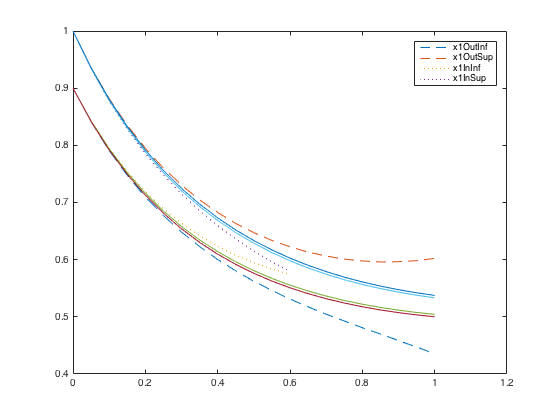
\epsfig{file=brusselator_x1_IA_AA.png,width=9cm,height=5cm}
%\end{center}
%\caption{Order 3 models, interval vs affine arithmetic \label{fig:brusselator_order3_t1}}
%\end{figure}

We use Taylor models of order 4 in time, and represent  in Figure~\ref{fig:brusselator_order4_x2_t10}, the inner and outer approximated flowpipes for variables $x_1$ and $x_2$, up to a maximum time $t=10$. The inner-approximations are represented in dashed lines, and the outer-approximations in plain lines. 

 We see that the width of the outer-approximation 
(external lines) remains indeed stable. 
Note that the width of the inner-approximation (internal dashed lines) can decrease until the inner-approximation becomes empty 
(this is the case for variable $x_2$ around $t=4$), but the width can still later be non-zero again. 
%At first look, this could appear as a bug in our implementation, but this is not the case. 
This is not a bug: this phenomenon is an illustration of the fact detailed in Section~\ref{practicalissues}, that when adding an improper with a proper interval to get the inner range of a variable, we can get a proper interval, which results in an empty inner-approximation (of the variable of interest - actually, you can note that on this example, the inner-approximations of the two variables do not become empty at the same time). 
This does not prevent us from carrying
on with the computation of the Taylor models~:  they can indeed give non-empty inner-approximations at later times, 
depending on the behavior of the Jacobian of the flow.    

%\begin{figure}[htbp]
%\begin{center}
%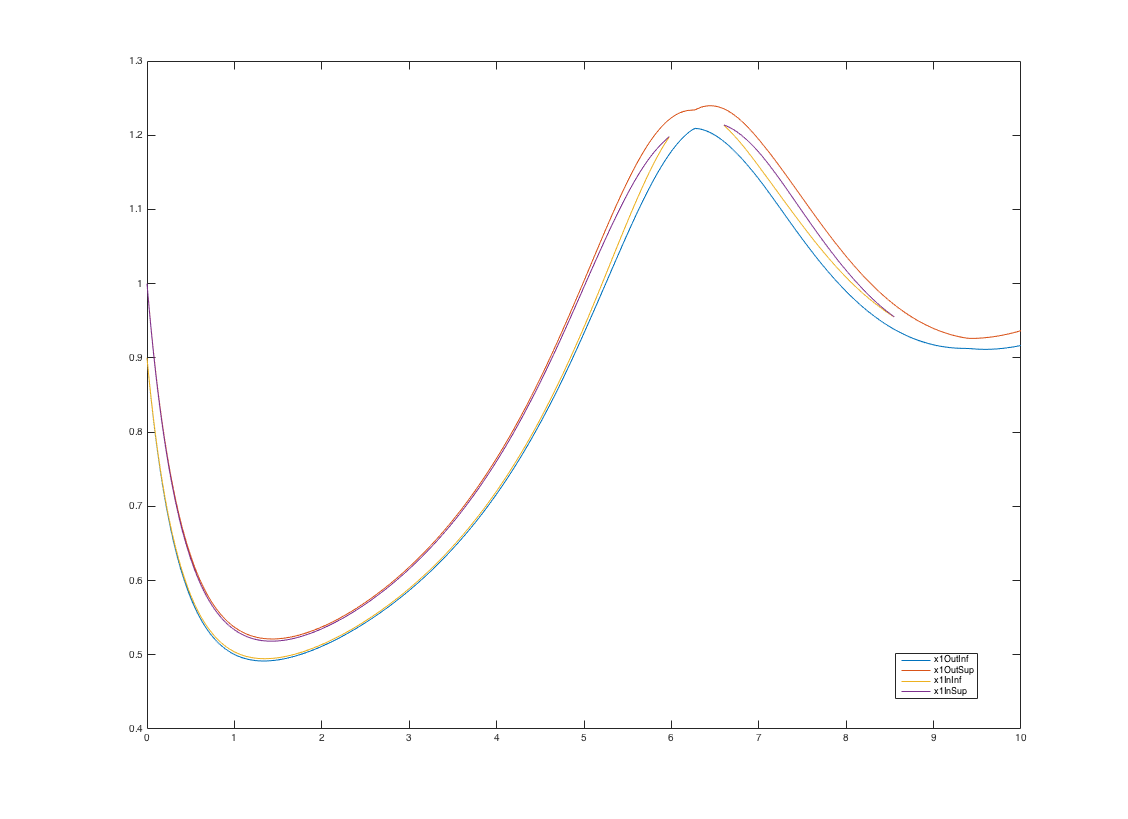
\epsfig{file=brusselator_x1_t10.png,clip=,width=9cm}
%\end{center}
%\caption{Brusselator (x1), evaluation of the Taylor models (order 4) with affine arithmetic \label{fig:brusselator_order4_x1_t10}}
%\end{figure}

\begin{figure}[htbp]
\begin{center}
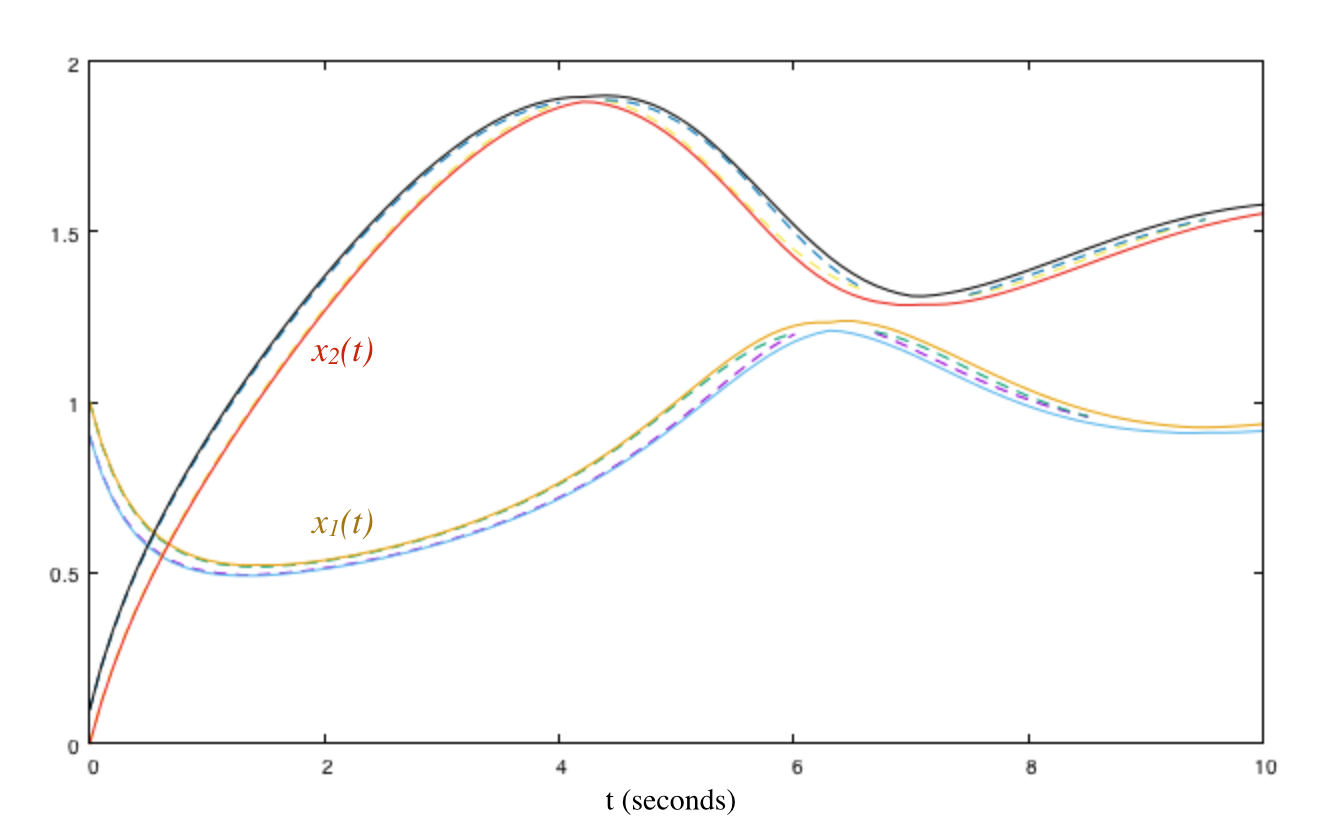
\epsfig{file=cav16_bruss_order4_x1x2b.png,width=9cm,height=5cm}
\end{center}
\caption{Brusselator ($x_1$ and $x_2$), Taylor models order 4 \label{fig:brusselator_order4_x2_t10}}
\end{figure}


%------------------------------------------------------------------------------------------------------------------------------------------------

% Exemple retiré car je n'arrive pas a bioen le traiter pour le moment
%\subsection{Car on the hill}
%\[ \left\{ 
%\begin{array}{lll} \dot x_1 & = & x_2 \\
%\dot x_2 & = & - 9.81 \sin(\frac{dg}{dx}(x_1))-0.7 x_2 + u
%\end{array}
%\right.
%\]
%where \[ g(x) = \frac{1}{2} (-\frac{1.1}{1.2} \cos(x) + \frac{1.2}{1.1} cos(1.1x)), \]
%the command $u$ is bounded in $[-2,2]$, the initial condition is $x_1(0) \in [-1,1]$, $x_2(0) \in [-1,1]$, 
%and we have limit conditions $x_1(t) \in [-1,13]$, $x_2(t) \in \R$ (conditions as in T. Le Mezo's document ``viability list of problems'')

%\SP{Si on peut montrer qu'on peut soit reussir a remonter la cite soit rester bloque, un peu comme T. Le Mezo a montre dans sa pres a brest, ca serait chouette. 
%Mais au moins dans l'implem matlab ca explose completement, mais relativement bizarrement: je ne suis qu'a moitié confiante sur l'AA dedans ...}
%}

\subsection{Comparisons to the related work}
\label{sec:exp_compar}
We provide in this section some elements of comparisons to the experimental results given in the related work~\cite{Underapproxflowpipes,underapprox16}.
Let us highlight that it is difficult to compare these methods in a fair manner, as evaluating the compared accuracy of these methods is difficult. 
Also, our implementation is preliminary (using fixed step of integration for instance), while some of the related work relies on the highly optimized 
interval solver for initial value problem {\tt VNODE-LP}~\cite{VNODELP}. 
%and on the other hand we only used a very basic Matlab implementation of our approach, whereas the related work relies on actual implementations,
%using optimized solvers such as VNode. In order to partially account for this overhead of our preliminary implementation, we will also compare in our experiments 
%the computation time of our inner approximated flowpipes, with the time taken by our implementation for the classical outer-approximation 
%of Taylor model flowpipes.  

%\ForAuthors{J'aime bien l'idee de comparer le cout du calcul sous-approx
%a celui de l'outer-approx du meme degre avec ton implem - tu le mets en
%remarque plus loin. Je pense qu'il faut l'expliquer un peu ici?
%Ok je ferai quand j'aurai integre ces resultats}

Among the examples studied in both ~\cite{Underapproxflowpipes} and \cite{underapprox16}, we first selected
the version of the Brusselator introduced in Section~\ref{sec:exp_bruss} as a representative of the systems of low degree. 
We chose as second example the following biological system, because of its higher degree (7), to investigate the way our approach scales. 
\begin{equation}
\dot{\left(\begin{array}{c}
x_1 \\
x_2 \\
x_3 \\
x_4 \\
x_5 \\
x_6 \\
x_7
\end{array}\right)} = \left(\begin{array}{c}
-0.4x_1+ a x_3x_4 \\
0.4x_1-x_2 \\
x_2- a x_3x_4 \\
a x_5x_6- a x_3x_4 \\
- a x_5x_6+ a x_3x_4 \\
0.5x_7- a x_5x_6 \\
-0.5x_7+ a x_5x_6
\end{array}\right)
\end{equation}
In this system, $a$ is a parameter which is taken, from our understanding, equal to 50 in \cite{Underapproxflowpipes} and to 5 in \cite{underapprox16}. 
We will use the corresponding value of the parameter when comparing to the related work.

\subsubsection{Comparison to \cite{Underapproxflowpipes}}
In  \cite{Underapproxflowpipes}, the  accuracy of computations is measured by the minimum width ratio 
\[ \gamma_{\min}=\min{\frac{\gamma_u(v)}{\gamma_o(v)}}, v \in V \]
where $V$ is a set of vectors, and $\gamma_u(v)$ and $\gamma_o(v)$ measure respectively the width of the inner-approximation and outer-approximation
in direction $v \in V$. 
Intuitively, the larger this ratio, the better the approximation. 
Our method naturally gives inner ranges for the projection of the flow system on its state variables. %(although we can also directly deduce from our Taylor models 
%an inner-approximation of the range of any linear function of these variables, and also define a joint range, as 
%already mentioned).
%\ForAuthors{Deja dit avant, on insiste ou pas?} 
We thus measure in our case the minimum over the state variables $x_i$ of our system of this ratio.  % \[ \gamma_{\min}=\min_{i}{\frac{\gamma_u(x_i)}{\gamma_o(x_i)}}, \]
%where the $x_i$ are the state variables of the system. 
We believe this corresponds to the measure that was used for experiments 
in~\cite{Underapproxflowpipes}, as they mention that the vectors are selected along the dimensions (axis-aligned).

%\ForAuthors{Sriram dit dans le dernier paragraph ``Results'' de [1], 
%pour $\gamma_{min}$ que ``The vectors are selected along the dimensions
%(axis-aligned).''? Donc ca serait comparable a nous?}
\paragraph{Comparison on the Brusselator}
The initial set taken in~\cite{Underapproxflowpipes}, defined by 
$x_1 \geq 0.9$, $x_2 \geq 0$, $x_1+x_2-1 \leq 0$, can be projected on $1 \geq x_1 \geq 0.9$, $0.1 \geq x_2 \geq 0$.
Naturally, this outer-approximation of the initial set is quite inaccurate, which will result in a lower quality of the inner-approximation
that must be taken into account in the comparison to the results of~\cite{Underapproxflowpipes}. In our approach, 
we could actually consider initial sets that are not given as intervals, for instance given as zonotopes 
(in the present case, we could use a zonotopic outer-approximation of the simplex),  
but we did not investigate this here. 


In ~\cite{Underapproxflowpipes}, the authors study the result for $t=3$ and $t=4$, with 4th order Taylor models and integration time step $h=0.02$. 
We choose, as they do, 4th order Taylor models,  and time step $h=0.02$. Our implementation until $t=4$
takes a total of $3.2$ seconds (to compute both outer and inner approximations), where \cite{Underapproxflowpipes} takes 89 seconds.
Our implementation is thus more than an order of magnitude quicker.
Note also that with our approach, taking order 3 Taylor models and a larger time step of 0.1, we still obtain results of very similar quality on $\gamma_{\min}$, in 0.25 seconds. 
Further decreasing the precision starts degrading the quality of results. 



On Figure~\ref{ex:width_sriram_bruss1}, we represent $\gamma_{\min}$ as a function of time, for a  time range 
extended to a maximum time of 10 in order to observe further behavior. 
We observe that at $t=3$, the relative width of the inner-approximation over the
outer-approximation is of order $0.7$, which is equal to the value given in Table~1 of \cite{Underapproxflowpipes}. 
However, this ratio decreases quickly, mostly due to the $x_2$ component, and at $t=4$, we get a ratio very close to $0.1$,
instead of $0.55$ as in~\cite{Underapproxflowpipes}. Indeed, $t=4$ is a time at which, as already noted in Section~\ref{sec:exp_bruss}, our 
inner-approximation of variable $x_2$ is temporarily of lower quality, even though the $x_1$ inner estimate
is still of high quality. We note that it is only temporary, as at further times the quality then improves and degrades again. 
\begin{figure}[htbp]
\begin{center}
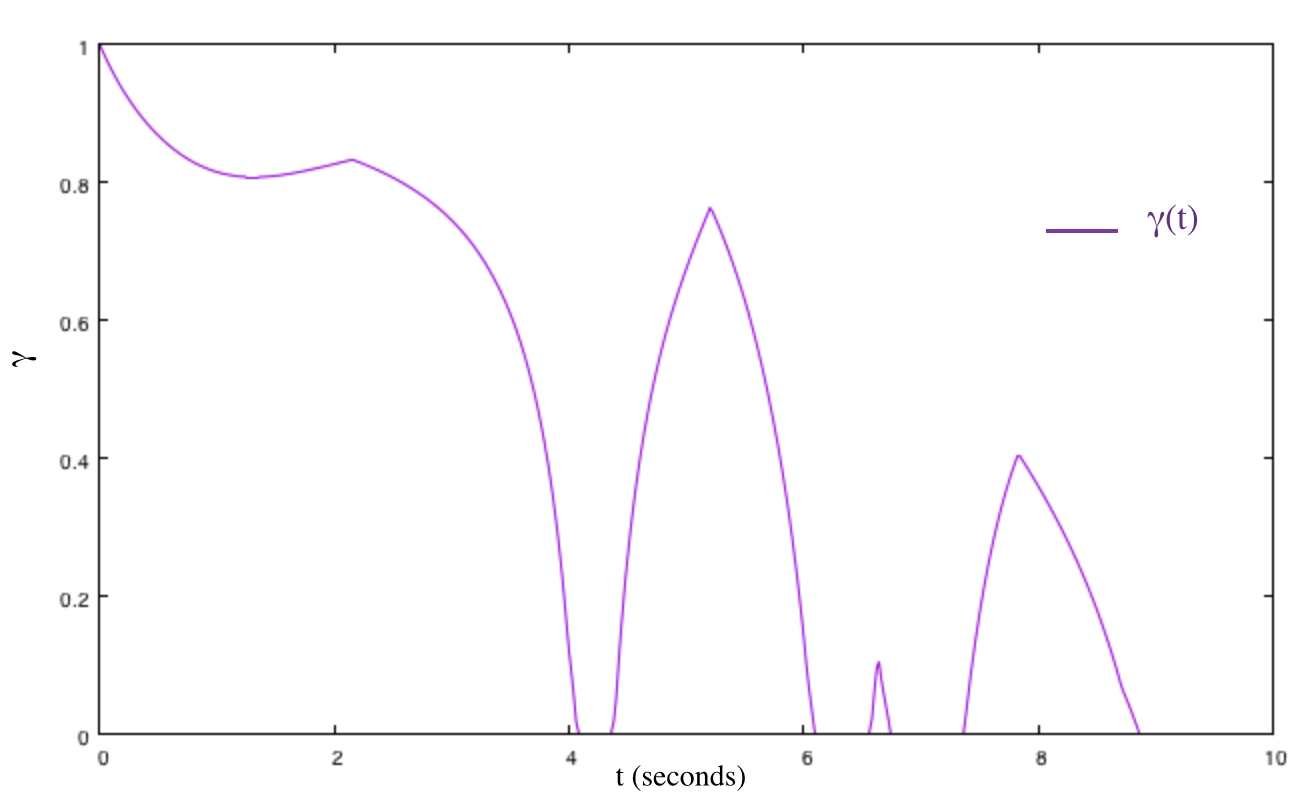
\epsfig{file=cav16_bruss_order4_gammab.png,width=9cm,height=5cm}
%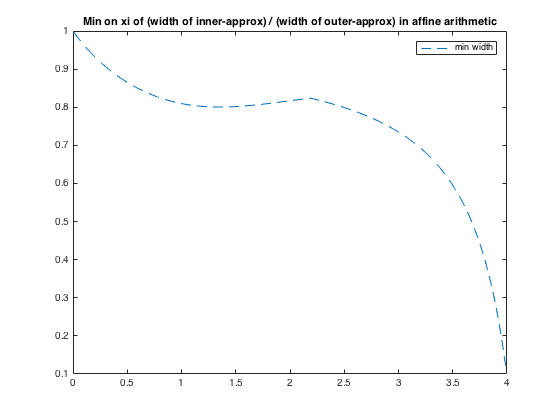
\epsfig{file=sriram_bruss_order4_t4_minwidth.png,width=9cm,height=5cm}
\end{center}
\caption{Evolution of $\gamma_{\min}$ with time \label{ex:width_sriram_bruss1} }
\end{figure}
On Figure~\ref{ex:width_sriram_bruss2}, we represent the evolution with time of the widths of the inner- and outer-approximations of $x_2$, 
the component that makes $\gamma_{\min}$ decrease drastically around $t=4$. We see that whenever the width of the inner-approximation on $x_2$ decreases 
to zero, the width of the outer-approximation is also strongly decreasing: the difference between these width remains 
almost stable. We also note again that the inner-approximation becoming empty at some point does not impact the behavior of the inner-approximation 
at further times. Finally, we note that this system looks quite stable, with solution widths that tend to decrease with time. This is of course a
difficult case for demonstrating  the inner-approximation, as its width naturally tends towards 0 due to the problem, as we note on 
Figure~\ref{ex:width_sriram_bruss2}. We advocate that inner and outer-approximations should be considered jointly in order to assess 
the behavior of a system. 

%This stable difference could be due to the outer-approximation of the flow starting from the center of our 
%initial value interval, and it could be interesting to use a higher order model to estimate this center, keeping lower order models for the Jacobian.
\begin{figure}[htbp]
\begin{center}
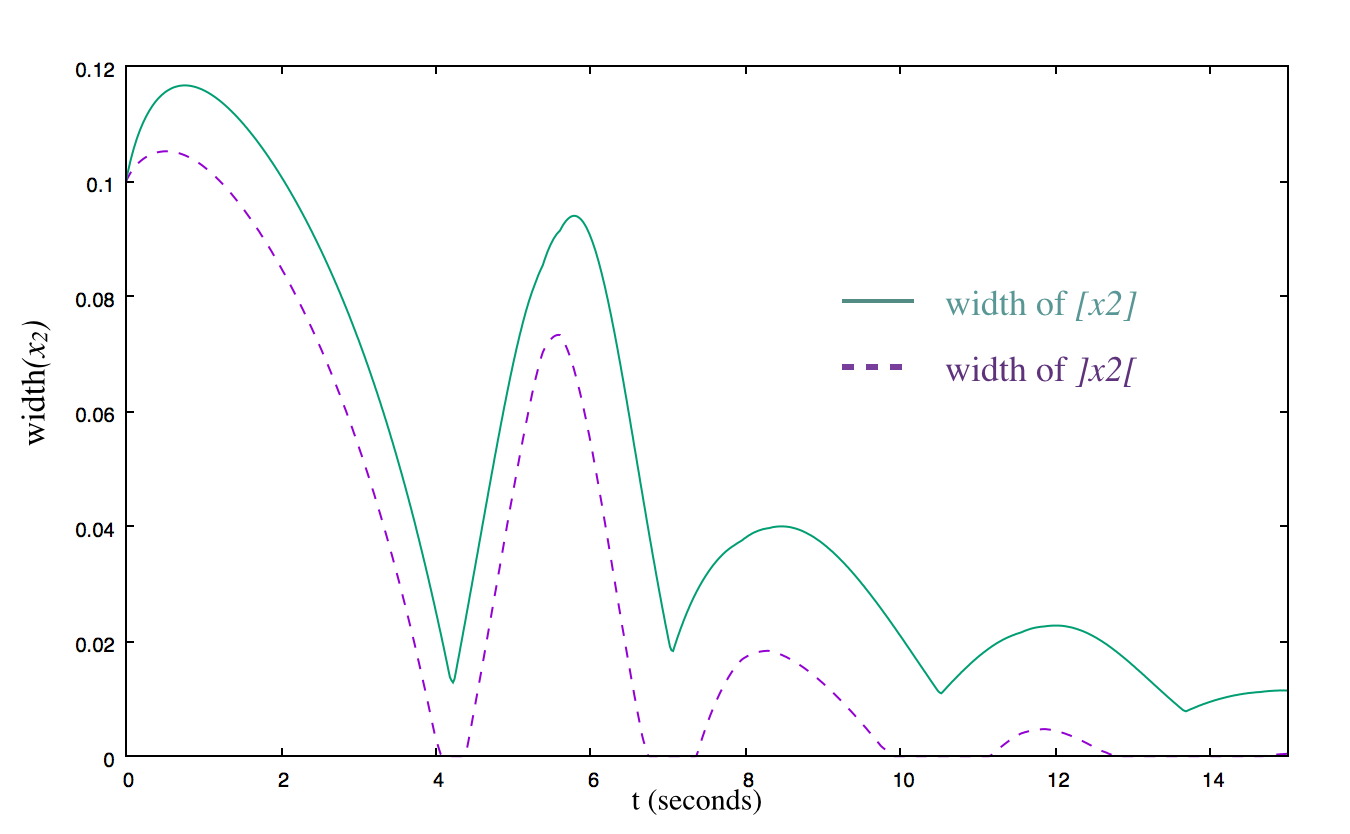
\epsfig{file=cav16_bruss_order4_width_x2b.png,width=9cm,height=5cm}
%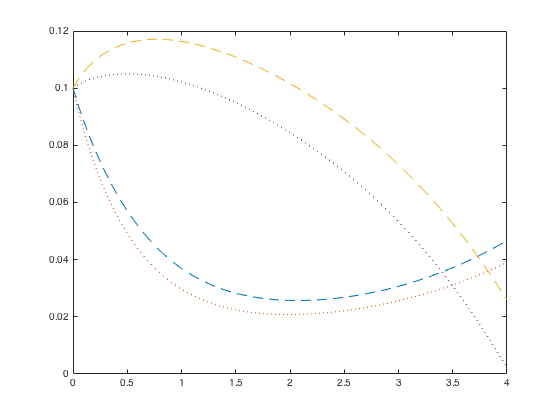
\epsfig{file=sriram_bruss_order4_t4_widthx1x2.png,width=9cm,height=5cm}
\end{center}
\caption{Evolution with time of the width of inner- and outer-approximations on $x_2$ \label{ex:width_sriram_bruss2} }
\end{figure}


\paragraph{Comparison on the biological system}
We now consider the biological system, with initial condition $\x_0 \in [0.1,0.1175] \times...\times [0.1,0.1175]$, which is an outer-approximation
of the simplex taken in  \cite{Underapproxflowpipes}. We compute inner and outer approximated flowpipes for time in [0,0.2], 
with order 5 Taylor Models and a step size of 0.01. The computation completes in 4.7 seconds, and we get as a measure of quality of the approximation 
$\gamma_{\min}(t=0.2) \approx 0.65$, which is this time a much better accuracy than the $\gamma_{\min}(t=0.2) = 0.25$ obtained in 632 seconds in  \cite{Underapproxflowpipes}. 
This seems to confirm that our approaches scales very well to high dimensional systems, with a very good accuracy. 

We also measure as an indication of the accuracy the mean value on the components $x_i$ of the distance between the inner and outer approximations $x_i^{in}$ and $x_i^{out}$,
computed as $$\sum_{i=1}^n \frac{\max(\sup(x_i^{out})-\sup(x_i^{in}),\inf(x_i^{in})- \inf(x_i^{out}))}{n}.$$
It gives an over-estimation of the error between the inner-approximation and the exact reachable state at time $t$: this value for $t=0.2$ is $4.10^{-3}$.

%elapsed_time_AA =  122.1330, step = 0.02, order 3
%elapsed_time_surapprox_AA =  39.6906


% je l'enleve pas passionnant 
%\begin{figure}
%\begin{center}
%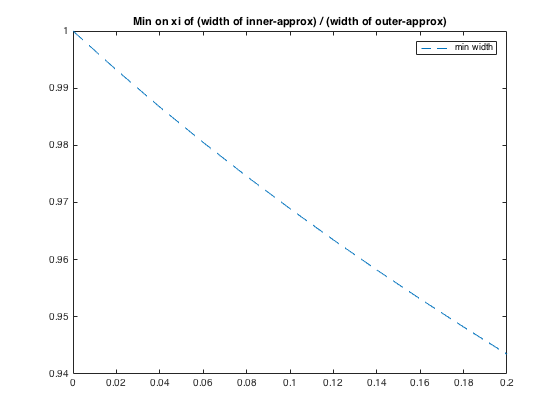
\epsfig{file=biological_sriram_002_order2_width.png,clip=,width=8cm}
%\end{center}
%\caption{Evolution of $\gamma_{\min}$ with time on the biological system}
%\label{ex:width_sriram_bio}
%\end{figure}

\subsubsection{Comparison to \cite{underapprox16}}
\paragraph{Comparison on the Brusselator}
In \cite{underapprox16} the authors take $X=[0.3, 0.4] \times [0.5, 0.7]$ for a time frame in [0,1.1], and a time step h=0.05. 
We compute the inner and outer-approximations, for same time step and with order 3 Taylor Models.
%Our implementation of the classical outer-approximated Taylor models only takes 16 seconds. 
%In Figure~\ref{fig:bruss_cav16}, we represent the inner and outer-approximations obtained for $x_1$ and $x_2$.  
%\begin{figure}[htbp]
%\begin{tabular}{cc}
%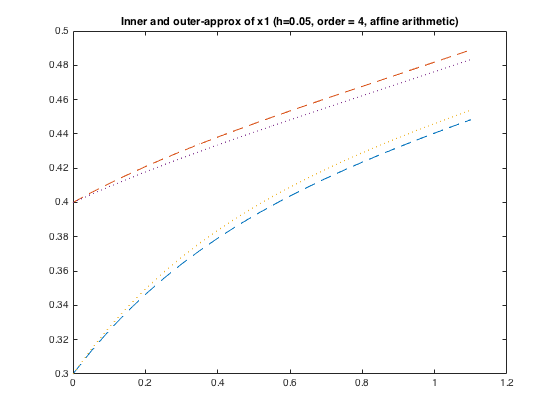
\epsfig{file=cav16_bruss_order4_x1.png,clip=,width=4cm}
%&
%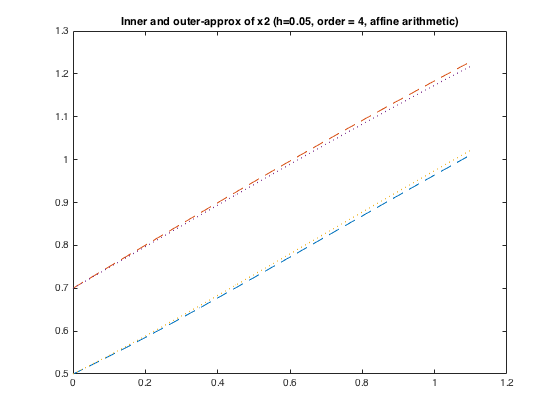
\epsfig{file=cav16_bruss_order4_x2.png,clip=,width=4cm}
%\end{tabular}
%\caption{Inner and outer approximations (order 4) for $x_1$ and $x_2$ \label{fig:bruss_cav16}}
%\ForAuthors{Trop petit?}
%\end{figure}
In \cite{underapprox16}, the accuracy of the result is estimated by a parameter $\epsilon_M$ that bounds the size of 
the boxes used to approximated the boundary of the exact reachable set, inside which they will look for an inner-approximation. 
We believe this parameter comparable in spirit 
to our measure of the maximum distance between the inner and the outer approximations. We can point 2 differences. First, in our case 
we compute the distance to the outer-approximation, which will always be greater than the distance to the exact reachable set.
Also, our understanding is that there are no guarantees in the method of \cite{underapprox16} on the actual distance from the inner-approximation itself 
to the reachable set, whereas our bounds are guaranteed. 

We measure obtain in 0.8 seconds a distance equal to 0.005 for $x_1$, and 0.01 for $x_2$, which is 10 times larger than the estimation 0.001 obtained 
in 55 seconds in \cite{underapprox16}. 
% However, choosing  higher order models or smaller time steps does not seem to improve much our distance measures. 



\paragraph{Comparison on the biological system}
We now consider the biological system, with, as in \cite{underapprox16}, a box initial condition $\x_0 \in [-0.015,0.001] \times...\times [-0.015,0.001]$. 
In order to compare our results to their backward estimate, we compute inner and outer approximated flowpipes on the reverse flow, 
for time in [0,0.2] , and use order 3 Taylor Models and a step size of 0.02. Our computation of the inner and outer approximated flowpipes takes 0.2 seconds. 
We get inner-approximations that always strictly contain the  ones of \cite{underapprox16}, which takes 0.67 seconds to compute. Our analysis is thus both 
faster and with better quality results. 
%$[  -0.01628536833380,   0.00103619844301]  [  -0.01833708041159,   0.00255842760143]  [  -0.01514208680158,   0.00416990950253]  [  -0.01488096912574,   0.00087696255375] 
%[  -0.01487744391170,   0.00088145048369]  [  -0.01492448895828,   0.00247920964913]  [  -0.01660493465136,   0.00105021396051] $
%to be compared to the always tighter (thus with lower quality) $[-0.0152,0.000]\times[-0.0169,0.0011]\times [-0.00140,0.0030]\times[-0.0141,0.0001]\times [-0.0141,0.0001]\times [-0.0138,0.0014]\times [-0.0155,0.0000]$
%of \cite{underapprox16}, which takes 0.67 seconds to compute.

Using as quality measure the measure of  \cite{Underapproxflowpipes} that computes the ratio $\gamma$ of the width of the inner-approximation over the width of the outer-approximation, 
here componentwise on the variables, and using our outer-approximation in both cases, we obtain for our approximation
$(\gamma_1,\ldots,\gamma_n)=(0.970,   0.999,   0.973,   0.938,   0.938,   0.970,   0.971)$, 
while with the results of \cite{underapprox16} we get the lower quality results
$(\gamma_1,\ldots,\gamma_n)=( 0.85,   0.86,   0.22,   0.84 ,  0.84 ,  0.85,   0.85)$.

We also compare our results with the outer-approximation computed by VNODE with a Taylor model of order 5. 
We represent on Figure~\ref{fig:histo} the upper bound for each of the 7 variables $x_i$ on the outer-approximation by VNode,  
our outer-approximation, our inner-approximation, and that of \cite{underapprox16}, in that order, from left to right.
\begin{figure}[htbp]
\begin{center}
%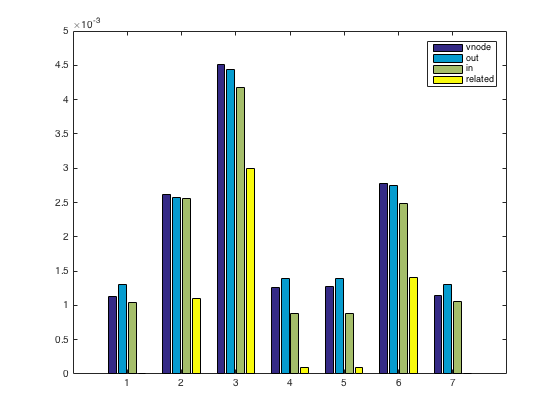
\epsfig{file=histo_sup.png,width=9cm,height=5cm}
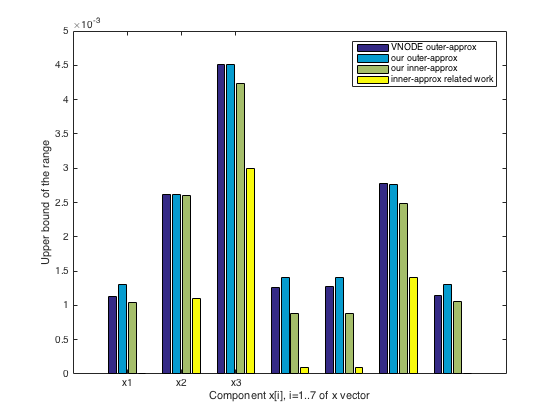
\epsfig{file=biological_matlab.png,width=9cm,height=5cm}
\end{center}
\caption{Upper bounds on inner and outer-approximations on the 7 variables of the biological system \label{fig:histo}}
\end{figure}
The results confirm that our inner-approximation (third bar of each group in the Figure, noted 'in') is generally very close to the outer-approximations (first two bars in each group),
while the inner-approximation of the related work (fourth bar, noted 'related') is of lower quality, and on some variables even absent (upper bound equal to zero).

%We get as width of inner-approximation on each component at time 0.2 the following:

%\begin{tabular}{l|c|c|c}
% & õur inner/outer & VNODE (order 20) &  inner\cite{underapprox16} \\
%Time & 115sec (36 for outer-approx only) & < 1 sec & 0.67 sec \\
%$x_1$ &  [  -0.016286,   0.0010362] / [  -0.016547,   0.0012979] & [-0.0166, 0.00131] & [-0.0152,0.000] 

%\end{tabular}

% $[   -0.01628,    0.00104]\times[   -0.01834,    0.00256]\times [   -0.01515,    0.00417]\times 
%[   -0.01489,    0.00088] \times[   -0.01488,    0.00089]\times[   -0.0150,    0.00248]\times [   -0.01661,    0.00106]$

%$[  -0.01628536833380,   0.00103619844301]  [  -0.01833708041159,   0.00255842760143]  [  -0.01514208680158,   0.00416990950253]  [  -0.01488096912574,   0.00087696255375] 
%[  -0.01487744391170,   0.00088145048369]  [  -0.01492448895828,   0.00247920964913]  [  -0.01660493465136,   0.00105021396051] $

%to be compared to the $[-0.0152,0.000]\times[-0.0169,0.0011]\times [-0.00140,0.0030]\times[-0.0141,0.0001]\times [-0.0141,0.0001]\times [-0.0138,0.0014]\times [-0.0155,0.0000]$
%Of \cite{underapprox16} .

%With VNODE at order 20 (with an execution time smaller than 1 second, which confirms the poor efficiency of our matlab implementation...) 
%$[-0.0166, 0.00131]
%[-0.0184, 0.00262]
%[-0.0154, 0.00451]
%[-0.0154, 0.00141]
%[-0.0154, 0.00141]
%[-0.0152, 0.00277]
%[-0.0169, 0.00131]$

%Our outer-approximation is $ [  -0.01654701249765,   0.00129784260686]  [  -0.01834542409233,   0.00256677128217]  [  -0.01540563322262,   0.00443345592357]
%[  -0.01539838418560,   0.00139437761361] [  -0.01538981256285,   0.00139381913484] [  -0.01519231394425,   0.00274703463510] [  -0.01686300688068,   0.00130828618983]$
%which look tighter than the VNODE order 20 results (???). 

%The mean distance from our inner-approximation to our outer-approximation, defined by $\sum_i=1^n \frac{|x_i^{out} - x_i^{in}|}{n}$, is thus equal to $3.10^{-4}$
% distance = sum(max(xouter.sup-xinner.sup,xinner.inf-xouter.inf))/7
%when the mean distance from the inner-approximation of \cite{underapprox16} to our approximation is $2.10^{-3}$ 

%the width of our outer-approximation is 
%   0.017844855104504   0.020912195374498   0.019839089146175   0.016792761799198   0.016783631697686   0.017939348579340   0.018171293070502

%the width of our inner-approx is
%   0.017321566776802   0.020895508013012   0.019311996304100   0.015757931679485   0.015758894395382   0.017403698607404   0.017655148611861

%width of inner / width of outer (same as sriram but componentwise)
%0.970675675165903   0.999202027277059   0.973431600705454   0.938376418835229   0.938944245157293   0.970141057822295   0.971595612010733

% 0.851786126084267   0.860741767072022   0.221784375662647   0.845602419054034   0.846062416989170   0.847299439707952   0.852993781997937

%\ForAuthors{A comparer au related workj, mais width de am surapporx (a recopier) < width de leur surapprox sur certains cas => wierd}

% [t,y] = ode23(@Bio_forode,[0 0.2],[-0.015; -0.015 ; -0.015; -0.015; -0.015; -0.015; -0.015]); => x3 sort de leur boite

%\paragraph{Comparaison to \cite{Underapproxflowpipes} on the biological system}

%for time in $[0,0.2]$, but again on differential initial conditions. 



%\subsection{Other examples}
%\paragraph{Moore-Greitzer model of a jet engine}
%\begin{equation}
%\dot{\left(\begin{array}{c}
%x \\
%y
%\end{array}\right)} = \left(\begin{array}{c}
%-y-1.5x^2-0.5x^3-0.5 \\
%3x-y
%\end{array}\right)
%\end{equation}
%The initial set is given by the simplex 
%$$X_0=\{(x,y) \in \R^2 | -x \leq -0.9 \wedge -y \leq -0.9\wedge x+y-2 \leq 0\}$$

%In \cite{Underapproxflowpipes}, two cases are considered : 
%\begin{itemize}
%\item computation of the inner and outer approximations of the reachable set at time
%$t=0.04$
%\item computation of the inner and outer approximations of the reachable set at times
%in [0,3] (using a step-size $\delta=0.02$)
%\end{itemize}

%\ForAuthors{Je rajoute les equations plus tard}

%\paragraph{Shimizu-Morioka}

%\paragraph{Steam governor}

%\paragraph{R\"ossler}


%\paragraph{Lorenz}

%\paragraph{Lotka-Volterra}
%(also from \cite{underapprox16}?)

%\begin{equation}
%\dot{\left(\begin{array}{c}
%x_1 \\
%x_2 \\
%x_3
%\end{array}\right)} = \left(\begin{array}{c}
%x_1x_2-x_1x_3 \\
%x_2x_3-x_2x_1 \\
%x_3x_1-x_3x_2
%\end{array}\right)
%\end{equation}

%\paragraph{Coupled Van der Pol}

%The next set of examples is taken from \cite{underapprox16}. 

%\paragraph{Electromechanical oscillation}

%\begin{equation}
%\dot{\left(\begin{array}{c}
%x \\
%y
%\end{array}\right)} = \left(\begin{array}{c}
%y \\
%0.2-0.7sin(x)-0.05y
%\end{array}\right)
%\end{equation}
%The initial set is given by $[-0.1,0.1]\times [2.9,3.1]$. We are looking at an 
%inner-approximation at times $t=0.5$ and $t=3$. 

%\paragraph{Van der Pol}

%\begin{equation}
%\dot{\left(\begin{array}{c}
%x_1 \\
%x_2
%\end{array}\right)} = \left(\begin{array}{c}
%x_2 \\
%-0.2(x^2_1-1)x_2-x_1
%\end{array}\right)
%\end{equation}

%\paragraph{Integrable systems}
%To make precision estimates of our method. 

%$$\dot{u}=u^2$$
%\noindent with $u(0)=u_0$. 
%Then $u=\frac{u_0}{1-u_0t}$

%The logistic equation :

%$$\dot{u}=\lambda u(1-u)$$
%\noindent with $u(0)=u_0$. Then
%$u(t)=\frac{u_0e^{\lambda t}}{1-u_0+u_0e^{\lambda t}}$.

%\ForAuthors{Pour $0 < u_0 < 1$ et $\lambda > 0$ par exemple, c'est une fonction decroissante
%en $u_0$ et $\lambda$ donc on trouve facilement les bornes!}

%\ForAuthors{Pas mal d'autres dans \url{http://www.math.umn.edu/~olver/am_/odz.pdf} mais les deux au dessus paraissent simples et raisonnables, surtout la 
%logistic equation?}

%$$\dot{y} = \frac{a}{\sqrt{y}}+y$$
%\noindent with $y(a)=1$
%Solution is :
%$$y(t)=\left(exp\left(\frac{3t}{2} - \frac{3a}{2} + log(a + 1)\right) - a\right)^{\frac{2}{3}}$$
%(from Mathworks - can find $y(0)$ and translate it into polynomial system?)

%\subsection{Conclusion}
%Resultats preliminaires qui peuvent ne pas sembler que positif mais a priori essentiellement dus a %la presente implem
%\ForAuthors{
%- comparaison sur / sous-approx => sous-approx competitive en complexite par rapport aux modeles de Taylor classiques\\
%- bon passage a l'echelle sur degre 7 ? \\
%- IA / AA laissant etendre que implem AA utilisee tres sous-optimale
%- un des interets est qu'on peut raffiner la precision (sur et sous-approximee) en montant en ordre a la demande, du style algo a pas ou ordre adaptatif par cette 
%estimation directe de l'erreur!
%}
%------------------------------------------------------------------------------------------------------------------------------------------------

%******************************************************************************
\section{Conclusion and future work}
%******************************************************************************
%
We presented an approach to compute inner-approxima\-ting flowpipes of uncertain ODEs, that extends in a simple way Taylor-based 
methods for outer-approximating flowpipes. We assessed the good behaviour of the inner compared to the classical outer-approximations, 
and demonstrated that the method scales very well to larger-order systems of ODEs. 
The joint computation of the inner and outer-approximating flowpipes gives us a bound on the error to the exact reachable 
set at each instant, that we can use if needed to dynamically refine the approximation by using higher order Taylor models or smaller step sizes. 
Indeed, accurate error estimation, which is usually a difficult task, is a direct outcome of our computation.
A natural future extension of the present work, is the inner-approximation of reachable sets 
in presence of guards and constraints, so as to handle general hybrid systems. Our approach allows us to inner-approximate 
not only the variables as demonstrated here, but also the projection on whatever function of these variables, not only at 
specific times like the related work, but as flowpipes, that can be used for detection of intersection. 
The symbolic information included in our model  when we evaluate the Taylor models with affine arithmetic, 
will allow us to use existing work on the inner-approximation 
of joint range of functions and constraint solving, as e.g.~\cite{DBLP:journals/constraints/IshiiGJ12}.  
%In that respect, our current Matlab prototype, while producing interesting results for the continuous case, does not allow us to 
%handle this symbolic information in a satisfying way, and some engineering improvement is needed and planned.

Among the main interests of inner-approximation is the possibility to falsify properties. Our mid-term objective in that respect, 
is to use the combination of inner and outer approximations to tackle the verification and falsification of temporal properties
of uncertain hybrid systems, along the lines of~\cite{falsification2,IshiiYG16}. 


Finally, this work can be applied to other, related problems. First, this can be applied
to backward reachability problems, such as the ones treated in e.g.~\cite{underapprox16}, by considering
the opposite vector field. Secondly, this can be applied to a particular backward 
reachability problem : the inner-approximation of region
of attractions, for which we should compare our method with existing work~\cite{DBLP:conf/nolcos/KordaHJ13}. 

\bibliographystyle{abbrv}
\bibliography{hscc2017}

\end{document}
